% report/ExpAmain000.tex
\documentclass[18pt,c]{beamer}
\makeatletter
\let\beamer@writeslidentry@miniframeson=\beamer@writeslidentry
\def\beamer@writeslidentry@miniframesoff{%
  \expandafter\beamer@ifempty\expandafter{\beamer@framestartpage}{}% does not happen normally
  {%else
    % removed \addtocontents commands
   \clearpage\beamer@notesactions%
  }
}
\newcommand*{\miniframeson}{\let\beamer@writeslidentry=\beamer@writeslidentry@miniframeson}
\newcommand*{\miniframesoff}{\let\beamer@writeslidentry=\beamer@writeslidentry@miniframesoff}
\makeatother
% yellow
\definecolor{goldenyellow}{rgb}{1.0, 0.87, 0.0}
\definecolor{electricyellow}{rgb}{1.0, 1.0, 0.0}
\definecolor{icterine}{rgb}{0.99, 0.97, 0.37}
\definecolor{flavescent}{rgb}{0.97, 0.91, 0.56}
\definecolor{lemon}{rgb}{1.0, 0.97, 0.0}
% orange
\definecolor{amber}{rgb}{1.0, 0.75, 0.0}
\definecolor{cadmiumorange}{rgb}{0.93, 0.53, 0.18}
\definecolor{internationalorange}{rgb}{1.0, 0.31, 0.0}
% red
\definecolor{ferrarired}{rgb}{1.0, 0.11, 0.0}
\definecolor{fireenginered}{rgb}{0.81, 0.09, 0.13}
\definecolor{cadmiumred}{rgb}{0.89, 0.0, 0.13}
% blue
\definecolor{ao}{rgb}{0.0, 0.5, 0.0}
\definecolor{babyblueeyes}{rgb}{0.63, 0.79, 0.95}
\definecolor{bleudefrance}{rgb}{0.19, 0.55, 0.91}
\definecolor{blue}{rgb}{0.0, 0.0, 1.0}
\definecolor{cobalt}{rgb}{0.0, 0.28, 0.67}
\definecolor{darkmidnightblue}{rgb}{0.0, 0.2, 0.4}
\definecolor{brandeisblue}{rgb}{0.0, 0.44, 1.0}
\definecolor{deepskyblue}{rgb}{0.0, 0.75, 1.0}
\definecolor{iris}{rgb}{0.35, 0.31, 0.81}
\definecolor{navyblue}{rgb}{0.0, 0.0, 0.5}
\definecolor{ultramarine}{rgb}{0.07, 0.04, 0.56}
\definecolor{electricultramarine}{rgb}{0.25, 0.0, 1.0}
% green
\definecolor{cadmiumgreen}{rgb}{0.0, 0.42, 0.24}
\definecolor{darkpastelgreen}{rgb}{0.01, 0.75, 0.24}
\usetheme{Berlin}
\usecolortheme{default}
\usefonttheme{default}
\setbeamercolor{structure}{fg=cadmiumgreen}
\setbeamerfont{frametitle}{size=\footnotesize}
\usepackage{graphicx}
\renewcommand{\topfraction}{1.0}
\renewcommand{\floatpagefraction}{1.0}
\begin{document}
\title{Report of Experiment ExpA. 3-Symmetry: Sequential versus Multicore for GP, GE, and GE by DE. }
\author{Andreas Geyer-Schulz}
\date{\today}
\begin{frame}
\titlepage
\end{frame}
\begin{frame}
\frametitle{Abstract}
This experiment compares sequential and multicore learning
with {\tt xegaRun} for the 3-symmetry problem with nand functions
by three different evolutionary algorithms:
grammar-based genetic programming, grammatical evolution,
and grammatical evolution by differential evolution.
Grammatical evolution by differential evolution is a
novel combination of grammatical evolution and differential evolution.%\end{abstract}
\end{frame}
\begin{frame}[t, allowframebreaks]
\frametitle{Contents}
\tableofcontents[subsubsectionstyle=hide]
\vfill
\end{frame}
% report/ExpAmain001.tex
\miniframeson
\section{Design of Experiment}
% report/ExpAmain002.tex
\begin{frame}
\vspace*{2mm}
\begin{block}{
Definitions
}
In a {\bf controlled computational experiment} the influence
of one or more control parameters on the outcome is studied with
regard to a systematic setting of a set of selected control parameters.
All other parameters must be known and held constant.
 
The experiment should be repeatable.
\end{block}
\end{frame}% report/ExpAmain003.tex
\begin{frame}
\vspace*{2mm}
\begin{block}{
Description of Experiment
}
The purpose of this computational experiment is
to compare sequential ({\tt executionModel="Sequential"})
and multicore ({\tt executionModel="MultiCore"}) processing
for each algorithm,
and to establish a performance ranking of the three algorithms
grammar-based genetic programming ({\tt algorithm="sgp"}),
grammatical evolution ({\tt algorithm="sge"}), and
grammatical evolution by differential evolution ({\tt algorithm="sgede"}).
 
The {\bf problem environment} is the 3-symmetry problem:
Finding a boolean expression (with the nand function)
which is TRUE for symmetric 3-bit strings.
 
The {\bf solver} used is {\tt xegaRun} from the R-package {\tt xega}.
 
The experiment consists of 6 treatments, namely the sequential and
multicore version of each of the 3 algorithms.
\end{block}
\end{frame}% report/ExpAmain004.tex
% ExpA
% Table: Common Parameters of Experiment ExpA
% Thu May  8 21:57:16 2025
 \begin{frame}
 \fontsize{8pt}{9pt}\selectfont
 \frametitle{ Common Parameters of Experiment ExpA }
% latex table generated in R 4.4.3 by xtable 1.8-4 package
% Thu May  8 21:57:16 2025
\begin{table}[ht]
\centering
\begin{tabular}{rr}
  \hline
 & Parameter Value \\ 
  \hline
Experiment & ExpA \\ 
  Problem.Environment & 3-Symmetry Problem \\ 
  Optimize & Minimize! \\ 
  Trials & 200 \\ 
  Max.Depth.of.DTs & 7 \\ 
  Grammar & Nand.txt \\ 
  Replay & 0 \\ 
  Evaluation.Method & Deterministic \\ 
  Verbose & 1 \\ 
  Semantics & byValue \\ 
  Report.Eval.Errors & TRUE \\ 
  Termination.Condition & AbsoluteError \\ 
  Termination.Eps & -0.1 \\ 
  Worst.Fitness & -8 \\ 
  Init.Gene & InitGene \\ 
   \hline
\end{tabular}
\caption{Common Parameters of Experiment ExpA (Part 1)} 
\end{table}

 \label{ExpACommonTable000.tex}  
 \end{frame}

 % Label:  \label{ExpACommonTable000.tex}  
% report/ExpAmain005.tex
% ExpA
% Table: Common Parameters of Experiment ExpA
% Thu May  8 21:57:16 2025
 \begin{frame}
 \fontsize{8pt}{9pt}\selectfont
 \frametitle{ Common Parameters of Experiment ExpA }
% latex table generated in R 4.4.3 by xtable 1.8-4 package
% Thu May  8 21:57:16 2025
\begin{table}[ht]
\centering
\begin{tabular}{rr}
  \hline
 & Parameter Value \\ 
  \hline
Codons & 120 \\ 
  Codon.Precision & LCM \\ 
  Population.Size & 400 \\ 
  Max.Generations & 1000 \\ 
  Crossover.Rate & 0.2 \\ 
  Mutation.Rate & 0.4 \\ 
  IV.Crossover.Rate & Const \\ 
  Crossover.Rate.2 & 0.4 \\ 
  IV.Mutation.Rate & Const \\ 
  Mutation.Rate.2 & 0.8 \\ 
   \hline
\end{tabular}
\caption{Common Parameters of Experiment ExpA (Part 2)} 
\end{table}

 \label{ExpACommonTable001.tex}  
 \end{frame}

 % Label:  \label{ExpACommonTable001.tex}  
% report/ExpAmain006.tex
% ExpA
% Table: Parameters of Treatments of Experiment ExpA
% Thu May  8 21:57:16 2025
 \begin{frame}
 \fontsize{8pt}{9pt}\selectfont
 \frametitle{ Parameters of Treatments of Experiment ExpA }
% latex table generated in R 4.4.3 by xtable 1.8-4 package
% Thu May  8 21:57:16 2025
\begin{table}[ht]
\centering
\begin{tabular}{rrrrr}
  \hline
 & Treatment & Algorithm & Execution Model & Gene Map \\ 
  \hline
1 & MCSGE & sge & MultiCore & Mod \\ 
  2 & MCSGP & sgp & MultiCore & Bin2Dec \\ 
  3 & MCSGV & sgede & MultiCore & Identity \\ 
  4 & SQSGE & sge & Sequential & Mod \\ 
  5 & SQSGP & sgp & Sequential & Bin2Dec \\ 
  6 & SQSGV & sgede & Sequential & Identity \\ 
   \hline
\end{tabular}
\caption{Parameters of Treatments of Experiment ExpA} 
\end{table}

 \label{ExpADifferentTable000.tex}  
 \end{frame}

 % Label:  \label{ExpADifferentTable000.tex}  
% report/ExpAmain007.tex
% ExpA
% Table: The Production Table of Experiment ExpA
% Thu May  8 21:57:16 2025
 \begin{frame}
 \fontsize{8pt}{9pt}\selectfont
 \frametitle{ The Production Table of Experiment ExpA }
% latex table generated in R 4.4.3 by xtable 1.8-4 package
% Thu May  8 21:57:16 2025
\begin{table}[ht]
\centering
\begin{tabular}{rrr}
  \hline
 & LHS & RHS \\ 
  \hline
1 & $<$fe$>$ & $<$f0$>$ \\ 
  2 & $<$fe$>$ & $<$f2$>$($<$fe$>$,$<$fe$>$) \\ 
  3 & $<$f0$>$ & D1 \\ 
  4 & $<$f0$>$ & D2 \\ 
  5 & $<$f0$>$ & D3 \\ 
  6 & $<$f2$>$ & NAND \\ 
   \hline
\end{tabular}
\caption{The Production Table of Experiment ExpA} 
\end{table}

 \label{ExpAGrammarTable000.tex}  
 \end{frame}

 % Label:  \label{ExpAGrammarTable000.tex}  
% report/ExpAmain008.tex
\begin{frame}
\vspace*{2mm}
\begin{block}{

}
The experiment has two control variables:
 
{\tt exectionModel} with 2 levels: {\tt "Sequential"} and {\tt "MultiCore"}.
 
{\tt algorithm} with 3 levels: {\tt "sgp"}, {\tt "sge"} and {\tt "sgede"} .
 
We investigate sequential versus multicore execution and
 
the performance of the three algorithms.
\end{block}
\end{frame}% report/ExpAmain009.tex
\miniframeson
\section{Exploratory Analysis}
% report/ExpAmain010.tex
\miniframeson
\subsection{Do we {\bf always} solve the 3 symmetry problem?}
% report/ExpAmain011.tex
\begin{frame}
\vspace*{2mm}
\begin{block}{
Observation
}
In this experiment, the 3-symmetry problem is {\bf not always} correctly solved.
 
{\bf Evidence:}
In all treatments of the grammatical evolution algorithm (MCSGE and SQSGE), 
in a few trials, non-optimal solutions were observed with a limit of 1000 generations.
See next table.
\end{block}
\end{frame}% report/ExpAmain012.tex
% ExpA
% Table: Fitness (Number of errors).
% Thu May  8 21:57:16 2025
 \begin{frame}
 \fontsize{8pt}{9pt}\selectfont
 \frametitle{ Fitness (Number of errors). }
% latex table generated in R 4.4.3 by xtable 1.8-4 package
% Thu May  8 21:57:16 2025
\begin{table}[ht]
\centering
\begin{tabular}{rrrrrrrr}
  \hline
 & Treatment & Trials & Variable & min & mean & sd & max \\ 
  \hline
1 & MCSGE & 200 & Fitness & 0.00 & 0.02 & 0.20 & 2.00 \\ 
  5 & MCSGP & 200 & Fitness & 0.00 & 0.00 & 0.00 & 0.00 \\ 
  9 & MCSGV & 200 & Fitness & 0.00 & 0.00 & 0.00 & 0.00 \\ 
  13 & SQSGE & 200 & Fitness & 0.00 & 0.01 & 0.07 & 1.00 \\ 
  17 & SQSGP & 200 & Fitness & 0.00 & 0.00 & 0.00 & 0.00 \\ 
  21 & SQSGV & 200 & Fitness & 0.00 & 0.00 & 0.00 & 0.00 \\ 
   \hline
\end{tabular}
\caption{Fitness (Number of errors).} 
\end{table}

 \label{ExpAStatsTable000.tex}  
 \end{frame}

 % Label:  \label{ExpAStatsTable000.tex}  
% report/ExpAmain013.tex
\begin{frame}
\vspace*{2mm}
\begin{block}{
Recommendation: New Experiment.
}
It is suggested to use the maximal number of generations as additional control variable.
The goal is to find the (conditional) probability that the optimal solution is found
given a resource constraint.
\end{block}
\end{frame}% report/ExpAmain014.tex
\miniframeson
\subsection{Time of Treatments in Seconds: }
% report/ExpAmain015.tex
% ExpA
% Figure: 3-Symmetry: Sequential versus Multicore for GP, GE, and GE by DE. 
% Thu May  8 21:57:16 2025
 \begin{frame}
 \frametitle{ 3-Symmetry: Sequential versus Multicore for GP, GE, and GE by DE.  }
 \begin{center}
\includegraphics[width=0.5\textwidth, angle=-90]
{ExpAboxplottSeconds000.eps}
 \end{center}
 \label{ExpAboxplottSeconds000.eps}  
 \end{frame}

% report/ExpAmain016.tex
% ExpA
% Table: Time (s).
% Thu May  8 21:57:16 2025
 \begin{frame}
 \fontsize{8pt}{9pt}\selectfont
 \frametitle{ Time (s). }
% latex table generated in R 4.4.3 by xtable 1.8-4 package
% Thu May  8 21:57:16 2025
\begin{table}[ht]
\centering
\begin{tabular}{rrrrrrrr}
  \hline
 & Treatment & Trials & Variable & min & mean & sd & max \\ 
  \hline
2 & MCSGE & 200 & Seconds & 0.50 & 12.95 & 30.61 & 224.75 \\ 
  6 & MCSGP & 200 & Seconds & 0.52 & 3.50 & 2.32 & 13.52 \\ 
  10 & MCSGV & 200 & Seconds & 1.86 & 32.84 & 30.21 & 169.25 \\ 
  14 & SQSGE & 200 & Seconds & 2.38 & 32.47 & 52.25 & 413.90 \\ 
  18 & SQSGP & 200 & Seconds & 2.18 & 10.70 & 7.42 & 40.17 \\ 
  22 & SQSGV & 200 & Seconds & 3.14 & 36.00 & 31.53 & 252.23 \\ 
   \hline
\end{tabular}
\caption{Time (s).} 
\end{table}

 \label{ExpAStatsTable001.tex}  
 \end{frame}

 % Label:  \label{ExpAStatsTable001.tex}  
% report/ExpAmain017.tex
% ExpA
% Figure: 3-Symmetry: Sequential versus Multicore for GP, GE, and GE by DE. 
% Thu May  8 21:57:16 2025
 \begin{frame}
 \frametitle{ 3-Symmetry: Sequential versus Multicore for GP, GE, and GE by DE.  }
 \begin{center}
\includegraphics[width=0.5\textwidth, angle=-90]
{ExpAboxplottSeconds001.eps}
 \end{center}
 \label{ExpAboxplottSeconds001.eps}  
 \end{frame}

% report/ExpAmain018.tex
\miniframeson
\subsection{Number of Generations of Treatments}
% report/ExpAmain019.tex
% ExpA
% Figure: 3-Symmetry: Sequential versus Multicore for GP, GE, and GE by DE. 
% Thu May  8 21:57:16 2025
 \begin{frame}
 \frametitle{ 3-Symmetry: Sequential versus Multicore for GP, GE, and GE by DE.  }
 \begin{center}
\includegraphics[width=0.5\textwidth, angle=-90]
{ExpAboxplottGenerations000.eps}
 \end{center}
 \label{ExpAboxplottGenerations000.eps}  
 \end{frame}

% report/ExpAmain020.tex
% ExpA
% Table: Generations
% Thu May  8 21:57:16 2025
 \begin{frame}
 \fontsize{8pt}{9pt}\selectfont
 \frametitle{ Generations }
% latex table generated in R 4.4.3 by xtable 1.8-4 package
% Thu May  8 21:57:16 2025
\begin{table}[ht]
\centering
\begin{tabular}{rrrrrrrr}
  \hline
 & Treatment & Trials & Variable & min & mean & sd & max \\ 
  \hline
3 & MCSGE & 200 & Generations & 1.00 & 53.83 & 142.45 & 1000.00 \\ 
  7 & MCSGP & 200 & Generations & 1.00 & 6.70 & 4.15 & 25.00 \\ 
  11 & MCSGV & 200 & Generations & 1.00 & 13.69 & 11.18 & 60.00 \\ 
  15 & SQSGE & 200 & Generations & 1.00 & 42.26 & 99.14 & 1000.00 \\ 
  19 & SQSGP & 200 & Generations & 1.00 & 6.70 & 4.38 & 21.00 \\ 
  23 & SQSGV & 200 & Generations & 1.00 & 14.93 & 12.03 & 91.00 \\ 
   \hline
\end{tabular}
\caption{Generations} 
\end{table}

 \label{ExpAStatsTable002.tex}  
 \end{frame}

 % Label:  \label{ExpAStatsTable002.tex}  
% report/ExpAmain021.tex
% ExpA
% Figure: 3-Symmetry: Sequential versus Multicore for GP, GE, and GE by DE. 
% Thu May  8 21:57:16 2025
 \begin{frame}
 \frametitle{ 3-Symmetry: Sequential versus Multicore for GP, GE, and GE by DE.  }
 \begin{center}
\includegraphics[width=0.5\textwidth, angle=-90]
{ExpAboxplottGenerations001.eps}
 \end{center}
 \label{ExpAboxplottGenerations001.eps}  
 \end{frame}

% report/ExpAmain022.tex
\miniframeson
\section{Multi-core or Sequential?}
% report/ExpAmain023.tex
\begin{frame}
\frametitle{
Should we prefer multi-core or sequential processing?
}
For each agorithm we have to test:
\begin{enumerate}
\item Is the multi-core version faster (in seconds) than the sequential version?
 
\item Do both of them need the same resources (in generations)?
\end{enumerate}
Multi-core processing is only preferable if it is faster (in seconds)
when running for the same number of generations.
 
The evaluation of the population of genes is parallelized.
\end{frame}% report/ExpAmain024.tex
\miniframeson
\subsection{Multi-core or sequential processing? Algorithm SGP}
% report/ExpAmain025.tex
% ExpA
% Table: Time in (s) (SGP)
% Thu May  8 21:57:16 2025
 \begin{frame}
 \fontsize{8pt}{9pt}\selectfont
 \frametitle{ Time in (s) (SGP) }
% latex table generated in R 4.4.3 by xtable 1.8-4 package
% Thu May  8 21:57:16 2025
\begin{table}[ht]
\centering
\begin{tabular}{rrrrrrrr}
  \hline
 & Treatment & Trials & Variable & min & mean & sd & max \\ 
  \hline
2 & MCSGP & 200 & Seconds & 0.52 & 3.50 & 2.32 & 13.52 \\ 
  6 & SQSGP & 200 & Seconds & 2.18 & 10.70 & 7.42 & 40.17 \\ 
   \hline
\end{tabular}
\caption{Time in (s) (SGP)} 
\end{table}

 \label{ExpAStatsTable003.tex}  
 \end{frame}

 % Label:  \label{ExpAStatsTable003.tex}  
% report/ExpAmain026.tex
% ExpA
% Table: Number of Generations (SGP)
% Thu May  8 21:57:16 2025
 \begin{frame}
 \fontsize{8pt}{9pt}\selectfont
 \frametitle{ Number of Generations (SGP) }
% latex table generated in R 4.4.3 by xtable 1.8-4 package
% Thu May  8 21:57:16 2025
\begin{table}[ht]
\centering
\begin{tabular}{rrrrrrrr}
  \hline
 & Treatment & Trials & Variable & min & mean & sd & max \\ 
  \hline
3 & MCSGP & 200 & Generations & 1.00 & 6.70 & 4.15 & 25.00 \\ 
  7 & SQSGP & 200 & Generations & 1.00 & 6.70 & 4.38 & 21.00 \\ 
   \hline
\end{tabular}
\caption{Number of Generations (SGP)} 
\end{table}

 \label{ExpAStatsTable004.tex}  
 \end{frame}

 % Label:  \label{ExpAStatsTable004.tex}  
% report/ExpAmain027.tex
\begin{frame}[t]
 \frametitle{Test of $H_{0}$: Mean of treatment MCSGP is less than mean of SQSGP of variable Seconds }
 \scriptsize
 For variable Seconds of treatments SQSGP and MCSGP of experiment ExpA:

\vspace{1mm}
{\bf Hypothesis 0}: mean(Seconds of SQSGP)=10.7 - mean(Seconds of MCSGP)=3.5 is equal or greater than 0.


 \begin{center} is tested at a significance level 0.05 against: \end{center}

{\bf Hypothesis 1}: mean(Seconds of SQSGP)=10.7 - mean(Seconds of MCSGP)=3.5 is less than 0.
\vspace{1mm}
\vspace{1mm}

 Outliers of treatment SQSGP  are not removed (coef=0).

 Outliers of treatment MCSGP  are not removed (coef=0).
\vspace{1mm}
 
 The test-statistic W of the Wilcoxon rank sum test with continuity correction is 34375 with a p-value of 1 .
 Since the p-value 1 is above the significance level $\alpha= 0.05 $,
 for variable Seconds of treatments SQSGP and MCSGP of experiment ExpA 
 {\bf Hypothesis 0}: mean(Seconds of SQSGP)=10.7 - mean(Seconds of MCSGP)=3.5 is equal or greater than 0.
is {\bf accepted}.

 \end{frame}
% report/ExpAmain028.tex
\begin{frame}[t]
 \frametitle{Test of $H_{0}$: Means of treatments SQSGP and MCSGP of variable Seconds are equal. }
 \scriptsize
 For variable Seconds of treatments SQSGP and MCSGP of experiment ExpA:

\vspace{1mm}
{\bf Hypothesis 0}: mean(Seconds of SQSGP)=10.7 - mean(Seconds of MCSGP)=3.5 is equal to 0.


 \begin{center} is tested at a significance level 0.05 against: \end{center}

{\bf Hypothesis 1}: mean(Seconds of SQSGP)=10.7 - mean(Seconds of MCSGP)=3.5 is not equal to 0.
\vspace{1mm}
\vspace{1mm}

 Outliers of treatment SQSGP  are not removed (coef=0).

 Outliers of treatment MCSGP  are not removed (coef=0).
\vspace{1mm}
 
 The test-statistic W of the Wilcoxon rank sum test with continuity correction is 34375 with a p-value of 0 .
 Since the p-value 0 is below the significance level $\alpha= 0.05 $,
 for variable Seconds of treatments SQSGP and MCSGP of experiment ExpA 
 {\bf Hypothesis 0}: mean(Seconds of SQSGP)=10.7 - mean(Seconds of MCSGP)=3.5 is equal to 0.
is {\bf rejected}.

 \end{frame}
% report/ExpAmain029.tex
\begin{frame}[t]
 \frametitle{Test of $H_{0}$: Means of treatments MCSGP and SQSGP of variable Generations are equal. }
 \scriptsize
 For variable Generations of treatments MCSGP and SQSGP of experiment ExpA:

\vspace{1mm}
{\bf Hypothesis 0}: mean(Generations of MCSGP)=6.41 - mean(Generations of SQSGP)=6.23 is equal to 0.


 \begin{center} is tested at a significance level 0.05 against: \end{center}

{\bf Hypothesis 1}: mean(Generations of MCSGP)=6.41 - mean(Generations of SQSGP)=6.23 is not equal to 0.
\vspace{1mm}
\vspace{1mm}

 4 outliers of treatment MCSGP are removed (coef=1.5).

 7 outliers of treatment SQSGP are removed (coef=1.5).
\vspace{1mm}
 
 The test-statistic W of the Wilcoxon rank sum test with continuity correction is 19458 with a p-value of 0.623 .
 Since the p-value 0.623 is above the significance level $\alpha= 0.05 $,
 for variable Generations of treatments MCSGP and SQSGP of experiment ExpA 
 {\bf Hypothesis 0}: mean(Generations of MCSGP)=6.41 - mean(Generations of SQSGP)=6.23 is equal to 0.
is {\bf accepted}.

 \end{frame}
% report/ExpAmain030.tex
\miniframeson
\subsection{Multi-core or sequential processing? Algorithm SGE}
% report/ExpAmain031.tex
% ExpA
% Table: Time in (s) (SGE)
% Thu May  8 21:57:16 2025
 \begin{frame}
 \fontsize{8pt}{9pt}\selectfont
 \frametitle{ Time in (s) (SGE) }
% latex table generated in R 4.4.3 by xtable 1.8-4 package
% Thu May  8 21:57:16 2025
\begin{table}[ht]
\centering
\begin{tabular}{rrrrrrrr}
  \hline
 & Treatment & Trials & Variable & min & mean & sd & max \\ 
  \hline
2 & MCSGE & 200 & Seconds & 0.50 & 12.95 & 30.61 & 224.75 \\ 
  6 & SQSGE & 200 & Seconds & 2.38 & 32.47 & 52.25 & 413.90 \\ 
   \hline
\end{tabular}
\caption{Time in (s) (SGE)} 
\end{table}

 \label{ExpAStatsTable005.tex}  
 \end{frame}

 % Label:  \label{ExpAStatsTable005.tex}  
% report/ExpAmain032.tex
% ExpA
% Table: Number of Generations (SGE)
% Thu May  8 21:57:16 2025
 \begin{frame}
 \fontsize{8pt}{9pt}\selectfont
 \frametitle{ Number of Generations (SGE) }
% latex table generated in R 4.4.3 by xtable 1.8-4 package
% Thu May  8 21:57:16 2025
\begin{table}[ht]
\centering
\begin{tabular}{rrrrrrrr}
  \hline
 & Treatment & Trials & Variable & min & mean & sd & max \\ 
  \hline
3 & MCSGE & 200 & Generations & 1.00 & 53.83 & 142.45 & 1000.00 \\ 
  7 & SQSGE & 200 & Generations & 1.00 & 42.26 & 99.14 & 1000.00 \\ 
   \hline
\end{tabular}
\caption{Number of Generations (SGE)} 
\end{table}

 \label{ExpAStatsTable006.tex}  
 \end{frame}

 % Label:  \label{ExpAStatsTable006.tex}  
% report/ExpAmain033.tex
\begin{frame}[t]
 \frametitle{Test of $H_{0}$: Mean of treatment MCSGE is less than mean of SQSGE of variable Seconds }
 \scriptsize
 For variable Seconds of treatments SQSGE and MCSGE of experiment ExpA:

\vspace{1mm}
{\bf Hypothesis 0}: mean(Seconds of SQSGE)=32.5 - mean(Seconds of MCSGE)=12.9 is equal or greater than 0.


 \begin{center} is tested at a significance level 0.05 against: \end{center}

{\bf Hypothesis 1}: mean(Seconds of SQSGE)=32.5 - mean(Seconds of MCSGE)=12.9 is less than 0.
\vspace{1mm}
\vspace{1mm}

 Outliers of treatment SQSGE  are not removed (coef=0).

 Outliers of treatment MCSGE  are not removed (coef=0).
\vspace{1mm}
 
 The test-statistic W of the Wilcoxon rank sum test with continuity correction is 33164 with a p-value of 1 .
 Since the p-value 1 is above the significance level $\alpha= 0.05 $,
 for variable Seconds of treatments SQSGE and MCSGE of experiment ExpA 
 {\bf Hypothesis 0}: mean(Seconds of SQSGE)=32.5 - mean(Seconds of MCSGE)=12.9 is equal or greater than 0.
is {\bf accepted}.

 \end{frame}
% report/ExpAmain034.tex
\begin{frame}[t]
 \frametitle{Test of $H_{0}$: Means of treatments SQSGE and MCSGE of variable Seconds are equal. }
 \scriptsize
 For variable Seconds of treatments SQSGE and MCSGE of experiment ExpA:

\vspace{1mm}
{\bf Hypothesis 0}: mean(Seconds of SQSGE)=32.5 - mean(Seconds of MCSGE)=12.9 is equal to 0.


 \begin{center} is tested at a significance level 0.05 against: \end{center}

{\bf Hypothesis 1}: mean(Seconds of SQSGE)=32.5 - mean(Seconds of MCSGE)=12.9 is not equal to 0.
\vspace{1mm}
\vspace{1mm}

 Outliers of treatment SQSGE  are not removed (coef=0).

 Outliers of treatment MCSGE  are not removed (coef=0).
\vspace{1mm}
 
 The test-statistic W of the Wilcoxon rank sum test with continuity correction is 33164 with a p-value of 0 .
 Since the p-value 0 is below the significance level $\alpha= 0.05 $,
 for variable Seconds of treatments SQSGE and MCSGE of experiment ExpA 
 {\bf Hypothesis 0}: mean(Seconds of SQSGE)=32.5 - mean(Seconds of MCSGE)=12.9 is equal to 0.
is {\bf rejected}.

 \end{frame}
% report/ExpAmain035.tex
\begin{frame}[t]
 \frametitle{Test of $H_{0}$: Means of treatments MCSGE and SQSGE of variable Generations are equal. }
 \scriptsize
 For variable Generations of treatments MCSGE and SQSGE of experiment ExpA:

\vspace{1mm}
{\bf Hypothesis 0}: mean(Generations of MCSGE)=17.4 - mean(Generations of SQSGE)=18.7 is equal to 0.


 \begin{center} is tested at a significance level 0.05 against: \end{center}

{\bf Hypothesis 1}: mean(Generations of MCSGE)=17.4 - mean(Generations of SQSGE)=18.7 is not equal to 0.
\vspace{1mm}
\vspace{1mm}

 23 outliers of treatment MCSGE are removed (coef=1.5).

 24 outliers of treatment SQSGE are removed (coef=1.5).
\vspace{1mm}
 
 The test-statistic W of the Wilcoxon rank sum test with continuity correction is 14638 with a p-value of 0.328 .
 Since the p-value 0.328 is above the significance level $\alpha= 0.05 $,
 for variable Generations of treatments MCSGE and SQSGE of experiment ExpA 
 {\bf Hypothesis 0}: mean(Generations of MCSGE)=17.4 - mean(Generations of SQSGE)=18.7 is equal to 0.
is {\bf accepted}.

 \end{frame}
% report/ExpAmain036.tex
\miniframeson
\subsection{Multi-core or sequential processing? Algorithm SGV}
% report/ExpAmain037.tex
% ExpA
% Table: Time in (s) (SGV)
% Thu May  8 21:57:16 2025
 \begin{frame}
 \fontsize{8pt}{9pt}\selectfont
 \frametitle{ Time in (s) (SGV) }
% latex table generated in R 4.4.3 by xtable 1.8-4 package
% Thu May  8 21:57:16 2025
\begin{table}[ht]
\centering
\begin{tabular}{rrrrrrrr}
  \hline
 & Treatment & Trials & Variable & min & mean & sd & max \\ 
  \hline
2 & MCSGV & 200 & Seconds & 1.86 & 32.84 & 30.21 & 169.25 \\ 
  6 & SQSGV & 200 & Seconds & 3.14 & 36.00 & 31.53 & 252.23 \\ 
   \hline
\end{tabular}
\caption{Time in (s) (SGV)} 
\end{table}

 \label{ExpAStatsTable007.tex}  
 \end{frame}

 % Label:  \label{ExpAStatsTable007.tex}  
% report/ExpAmain038.tex
% ExpA
% Table: Number of Generations (SGV)
% Thu May  8 21:57:16 2025
 \begin{frame}
 \fontsize{8pt}{9pt}\selectfont
 \frametitle{ Number of Generations (SGV) }
% latex table generated in R 4.4.3 by xtable 1.8-4 package
% Thu May  8 21:57:16 2025
\begin{table}[ht]
\centering
\begin{tabular}{rrrrrrrr}
  \hline
 & Treatment & Trials & Variable & min & mean & sd & max \\ 
  \hline
3 & MCSGV & 200 & Generations & 1.00 & 13.69 & 11.18 & 60.00 \\ 
  7 & SQSGV & 200 & Generations & 1.00 & 14.93 & 12.03 & 91.00 \\ 
   \hline
\end{tabular}
\caption{Number of Generations (SGV)} 
\end{table}

 \label{ExpAStatsTable008.tex}  
 \end{frame}

 % Label:  \label{ExpAStatsTable008.tex}  
% report/ExpAmain039.tex
\begin{frame}[t]
 \frametitle{Test of $H_{0}$: Mean of treatment MCSGV is less than mean of SQSGV of variable Seconds }
 \scriptsize
 For variable Seconds of treatments SQSGV and MCSGV of experiment ExpA:

\vspace{1mm}
{\bf Hypothesis 0}: mean(Seconds of SQSGV)=36 - mean(Seconds of MCSGV)=32.8 is equal or greater than 0.


 \begin{center} is tested at a significance level 0.05 against: \end{center}

{\bf Hypothesis 1}: mean(Seconds of SQSGV)=36 - mean(Seconds of MCSGV)=32.8 is less than 0.
\vspace{1mm}
\vspace{1mm}

 Outliers of treatment SQSGV  are not removed (coef=0).

 Outliers of treatment MCSGV  are not removed (coef=0).
\vspace{1mm}
 
 The test-statistic W of the Wilcoxon rank sum test with continuity correction is 21854 with a p-value of 0.946 .
 Since the p-value 0.946 is above the significance level $\alpha= 0.05 $,
 for variable Seconds of treatments SQSGV and MCSGV of experiment ExpA 
 {\bf Hypothesis 0}: mean(Seconds of SQSGV)=36 - mean(Seconds of MCSGV)=32.8 is equal or greater than 0.
is {\bf accepted}.

 \end{frame}
% report/ExpAmain040.tex
\begin{frame}[t]
 \frametitle{Test of $H_{0}$: Means of treatments SQSGV and MCSGV of variable Seconds are equal. }
 \scriptsize
 For variable Seconds of treatments SQSGV and MCSGV of experiment ExpA:

\vspace{1mm}
{\bf Hypothesis 0}: mean(Seconds of SQSGV)=36 - mean(Seconds of MCSGV)=32.8 is equal to 0.


 \begin{center} is tested at a significance level 0.05 against: \end{center}

{\bf Hypothesis 1}: mean(Seconds of SQSGV)=36 - mean(Seconds of MCSGV)=32.8 is not equal to 0.
\vspace{1mm}
\vspace{1mm}

 Outliers of treatment SQSGV  are not removed (coef=0).

 Outliers of treatment MCSGV  are not removed (coef=0).
\vspace{1mm}
 
 The test-statistic W of the Wilcoxon rank sum test with continuity correction is 21854 with a p-value of 0.109 .
 Since the p-value 0.109 is above the significance level $\alpha= 0.05 $,
 for variable Seconds of treatments SQSGV and MCSGV of experiment ExpA 
 {\bf Hypothesis 0}: mean(Seconds of SQSGV)=36 - mean(Seconds of MCSGV)=32.8 is equal to 0.
is {\bf accepted}.

 \end{frame}
% report/ExpAmain041.tex
\begin{frame}[t]
 \frametitle{Test of $H_{0}$: Means of treatments MCSGV and SQSGV of variable Generations are equal. }
 \scriptsize
 For variable Generations of treatments MCSGV and SQSGV of experiment ExpA:

\vspace{1mm}
{\bf Hypothesis 0}: mean(Generations of MCSGV)=12.7 - mean(Generations of SQSGV)=13.8 is equal to 0.


 \begin{center} is tested at a significance level 0.05 against: \end{center}

{\bf Hypothesis 1}: mean(Generations of MCSGV)=12.7 - mean(Generations of SQSGV)=13.8 is not equal to 0.
\vspace{1mm}
\vspace{1mm}

 6 outliers of treatment MCSGV are removed (coef=1.5).

 5 outliers of treatment SQSGV are removed (coef=1.5).
\vspace{1mm}
 
 The test-statistic W of the Wilcoxon rank sum test with continuity correction is 17416 with a p-value of 0.176 .
 Since the p-value 0.176 is above the significance level $\alpha= 0.05 $,
 for variable Generations of treatments MCSGV and SQSGV of experiment ExpA 
 {\bf Hypothesis 0}: mean(Generations of MCSGV)=12.7 - mean(Generations of SQSGV)=13.8 is equal to 0.
is {\bf accepted}.

 \end{frame}
% report/ExpAmain042.tex
\miniframeson
\subsection{Multi-core or sequential processing? Summary}
% report/ExpAmain043.tex
\begin{frame}
\frametitle{
Multi-core or sequential processing?
}
\begin{center}
\begin{tabular}{c|ccc}
\hline
  Multi-core             & SGP & SGE & SGV \\
\hline
  ... equal speed or faster ?  & yes & yes & yes \\
  ... equal speed?       &  no &  no & yes \\
  ... same resources?    & yes & yes & yes \\
\hline
\end{tabular}
\end{center}
 
\vspace{2mm} 
\begin{itemize}
\item {\bf Recommendation:} Use multi-core for 
       population sizes larger than 400.
\item {\bf New experiment:} Population size as control variable.
\end{itemize}
\end{frame}% report/ExpAmain044.tex
\miniframeson
\section{Which algorithm?}
% report/ExpAmain045.tex
\begin{frame}
\frametitle{
Which algorithm?
}
We compare the performance (time and resources used) of the three algorithms
\begin{enumerate}
\item for sequential processing and 
 
\item for multi-core processing.
\end{enumerate}
 
The evaluation of the population of genes is parallelized.
\end{frame}% report/ExpAmain046.tex
\miniframeson
\subsection{Which algorithm? Sequential processing.}
% report/ExpAmain047.tex
% ExpA
% Table: Time in (s) (Sequential)
% Thu May  8 21:57:17 2025
 \begin{frame}
 \fontsize{8pt}{9pt}\selectfont
 \frametitle{ Time in (s) (Sequential) }
% latex table generated in R 4.4.3 by xtable 1.8-4 package
% Thu May  8 21:57:17 2025
\begin{table}[ht]
\centering
\begin{tabular}{rrrrrrrr}
  \hline
 & Treatment & Trials & Variable & min & mean & sd & max \\ 
  \hline
2 & SQSGE & 200 & Seconds & 2.38 & 32.47 & 52.25 & 413.90 \\ 
  6 & SQSGP & 200 & Seconds & 2.18 & 10.70 & 7.42 & 40.17 \\ 
  10 & SQSGV & 200 & Seconds & 3.14 & 36.00 & 31.53 & 252.23 \\ 
   \hline
\end{tabular}
\caption{Time in (s) (Sequential)} 
\end{table}

 \label{ExpAStatsTable009.tex}  
 \end{frame}

 % Label:  \label{ExpAStatsTable009.tex}  
% report/ExpAmain048.tex
\begin{frame}[t]
 \frametitle{Test of $H_{0}$: Mean of treatment SQSGE is greater than mean of SQSGP of variable Seconds }
 \scriptsize
 For variable Seconds of treatments SQSGP and SQSGE of experiment ExpA:

\vspace{1mm}
{\bf Hypothesis 0}: mean(Seconds of SQSGP)=10.7 - mean(Seconds of SQSGE)=32.5 is equal or less than 0.


 \begin{center} is tested at a significance level 0.05 against: \end{center}

{\bf Hypothesis 1}: mean(Seconds of SQSGP)=10.7 - mean(Seconds of SQSGE)=32.5 is greater than 0.
\vspace{1mm}
\vspace{1mm}

 Outliers of treatment SQSGP  are not removed (coef=0).

 Outliers of treatment SQSGE  are not removed (coef=0).
\vspace{1mm}
 
 The test-statistic W of the Wilcoxon rank sum test with continuity correction is 9899 with a p-value of 1 .
 Since the p-value 1 is above the significance level $\alpha= 0.05 $,
 for variable Seconds of treatments SQSGP and SQSGE of experiment ExpA 
 {\bf Hypothesis 0}: mean(Seconds of SQSGP)=10.7 - mean(Seconds of SQSGE)=32.5 is equal or less than 0.
is {\bf accepted}.

 \end{frame}
% report/ExpAmain049.tex
\begin{frame}[t]
 \frametitle{Test of $H_{0}$: Means of treatments SQSGP and SQSGE of variable Seconds are equal. }
 \scriptsize
 For variable Seconds of treatments SQSGP and SQSGE of experiment ExpA:

\vspace{1mm}
{\bf Hypothesis 0}: mean(Seconds of SQSGP)=10.7 - mean(Seconds of SQSGE)=32.5 is equal to 0.


 \begin{center} is tested at a significance level 0.05 against: \end{center}

{\bf Hypothesis 1}: mean(Seconds of SQSGP)=10.7 - mean(Seconds of SQSGE)=32.5 is not equal to 0.
\vspace{1mm}
\vspace{1mm}

 Outliers of treatment SQSGP  are not removed (coef=0).

 Outliers of treatment SQSGE  are not removed (coef=0).
\vspace{1mm}
 
 The test-statistic W of the Wilcoxon rank sum test with continuity correction is 9899 with a p-value of 0 .
 Since the p-value 0 is below the significance level $\alpha= 0.05 $,
 for variable Seconds of treatments SQSGP and SQSGE of experiment ExpA 
 {\bf Hypothesis 0}: mean(Seconds of SQSGP)=10.7 - mean(Seconds of SQSGE)=32.5 is equal to 0.
is {\bf rejected}.

 \end{frame}
% report/ExpAmain050.tex
\begin{frame}[t]
 \frametitle{Test of $H_{0}$: Mean of treatment SQSGV is greater than mean of SQSGP of variable Seconds }
 \scriptsize
 For variable Seconds of treatments SQSGP and SQSGV of experiment ExpA:

\vspace{1mm}
{\bf Hypothesis 0}: mean(Seconds of SQSGP)=10.7 - mean(Seconds of SQSGV)=36 is equal or less than 0.


 \begin{center} is tested at a significance level 0.05 against: \end{center}

{\bf Hypothesis 1}: mean(Seconds of SQSGP)=10.7 - mean(Seconds of SQSGV)=36 is greater than 0.
\vspace{1mm}
\vspace{1mm}

 Outliers of treatment SQSGP  are not removed (coef=0).

 Outliers of treatment SQSGV  are not removed (coef=0).
\vspace{1mm}
 
 The test-statistic W of the Wilcoxon rank sum test with continuity correction is 7796 with a p-value of 1 .
 Since the p-value 1 is above the significance level $\alpha= 0.05 $,
 for variable Seconds of treatments SQSGP and SQSGV of experiment ExpA 
 {\bf Hypothesis 0}: mean(Seconds of SQSGP)=10.7 - mean(Seconds of SQSGV)=36 is equal or less than 0.
is {\bf accepted}.

 \end{frame}
% report/ExpAmain051.tex
\begin{frame}[t]
 \frametitle{Test of $H_{0}$: Means of treatments SQSGP and SQSGV of variable Seconds are equal. }
 \scriptsize
 For variable Seconds of treatments SQSGP and SQSGV of experiment ExpA:

\vspace{1mm}
{\bf Hypothesis 0}: mean(Seconds of SQSGP)=10.7 - mean(Seconds of SQSGV)=36 is equal to 0.


 \begin{center} is tested at a significance level 0.05 against: \end{center}

{\bf Hypothesis 1}: mean(Seconds of SQSGP)=10.7 - mean(Seconds of SQSGV)=36 is not equal to 0.
\vspace{1mm}
\vspace{1mm}

 Outliers of treatment SQSGP  are not removed (coef=0).

 Outliers of treatment SQSGV  are not removed (coef=0).
\vspace{1mm}
 
 The test-statistic W of the Wilcoxon rank sum test with continuity correction is 7796 with a p-value of 0 .
 Since the p-value 0 is below the significance level $\alpha= 0.05 $,
 for variable Seconds of treatments SQSGP and SQSGV of experiment ExpA 
 {\bf Hypothesis 0}: mean(Seconds of SQSGP)=10.7 - mean(Seconds of SQSGV)=36 is equal to 0.
is {\bf rejected}.

 \end{frame}
% report/ExpAmain052.tex
\begin{frame}[t]
 \frametitle{Test of $H_{0}$: Mean of treatment SQSGV is greater than mean of SQSGE of variable Seconds }
 \scriptsize
 For variable Seconds of treatments SQSGE and SQSGV of experiment ExpA:

\vspace{1mm}
{\bf Hypothesis 0}: mean(Seconds of SQSGE)=32.5 - mean(Seconds of SQSGV)=36 is equal or less than 0.


 \begin{center} is tested at a significance level 0.05 against: \end{center}

{\bf Hypothesis 1}: mean(Seconds of SQSGE)=32.5 - mean(Seconds of SQSGV)=36 is greater than 0.
\vspace{1mm}
\vspace{1mm}

 Outliers of treatment SQSGE  are not removed (coef=0).

 Outliers of treatment SQSGV  are not removed (coef=0).
\vspace{1mm}
 
 The test-statistic W of the Wilcoxon rank sum test with continuity correction is 15850 with a p-value of 1 .
 Since the p-value 1 is above the significance level $\alpha= 0.05 $,
 for variable Seconds of treatments SQSGE and SQSGV of experiment ExpA 
 {\bf Hypothesis 0}: mean(Seconds of SQSGE)=32.5 - mean(Seconds of SQSGV)=36 is equal or less than 0.
is {\bf accepted}.

 \end{frame}
% report/ExpAmain053.tex
\begin{frame}[t]
 \frametitle{Test of $H_{0}$: Means of treatments SQSGE and SQSGV of variable Seconds are equal. }
 \scriptsize
 For variable Seconds of treatments SQSGE and SQSGV of experiment ExpA:

\vspace{1mm}
{\bf Hypothesis 0}: mean(Seconds of SQSGE)=32.5 - mean(Seconds of SQSGV)=36 is equal to 0.


 \begin{center} is tested at a significance level 0.05 against: \end{center}

{\bf Hypothesis 1}: mean(Seconds of SQSGE)=32.5 - mean(Seconds of SQSGV)=36 is not equal to 0.
\vspace{1mm}
\vspace{1mm}

 Outliers of treatment SQSGE  are not removed (coef=0).

 Outliers of treatment SQSGV  are not removed (coef=0).
\vspace{1mm}
 
 The test-statistic W of the Wilcoxon rank sum test with continuity correction is 15850 with a p-value of 0.00033 .
 Since the p-value 0.00033 is below the significance level $\alpha= 0.05 $,
 for variable Seconds of treatments SQSGE and SQSGV of experiment ExpA 
 {\bf Hypothesis 0}: mean(Seconds of SQSGE)=32.5 - mean(Seconds of SQSGV)=36 is equal to 0.
is {\bf rejected}.

 \end{frame}
% report/ExpAmain054.tex
\miniframeson
\subsection{Which algorithm? Sequential processing. Generations.}
% report/ExpAmain055.tex
% ExpA
% Table: Number of Generations (Sequential)
% Thu May  8 21:57:17 2025
 \begin{frame}
 \fontsize{8pt}{9pt}\selectfont
 \frametitle{ Number of Generations (Sequential) }
% latex table generated in R 4.4.3 by xtable 1.8-4 package
% Thu May  8 21:57:17 2025
\begin{table}[ht]
\centering
\begin{tabular}{rrrrrrrr}
  \hline
 & Treatment & Trials & Variable & min & mean & sd & max \\ 
  \hline
3 & SQSGE & 200 & Generations & 1.00 & 42.26 & 99.14 & 1000.00 \\ 
  7 & SQSGP & 200 & Generations & 1.00 & 6.70 & 4.38 & 21.00 \\ 
  11 & SQSGV & 200 & Generations & 1.00 & 14.93 & 12.03 & 91.00 \\ 
   \hline
\end{tabular}
\caption{Number of Generations (Sequential)} 
\end{table}

 \label{ExpAStatsTable010.tex}  
 \end{frame}

 % Label:  \label{ExpAStatsTable010.tex}  
% report/ExpAmain056.tex
\begin{frame}[t]
 \frametitle{Test of $H_{0}$: Mean of treatment SQSGE is greater than mean of SQSGP of variable Generations }
 \scriptsize
 For variable Generations of treatments SQSGP and SQSGE of experiment ExpA:

\vspace{1mm}
{\bf Hypothesis 0}: mean(Generations of SQSGP)=6.7 - mean(Generations of SQSGE)=42.3 is equal or less than 0.


 \begin{center} is tested at a significance level 0.05 against: \end{center}

{\bf Hypothesis 1}: mean(Generations of SQSGP)=6.7 - mean(Generations of SQSGE)=42.3 is greater than 0.
\vspace{1mm}
\vspace{1mm}

 Outliers of treatment SQSGP  are not removed (coef=0).

 Outliers of treatment SQSGE  are not removed (coef=0).
\vspace{1mm}
 
 The test-statistic W of the Wilcoxon rank sum test with continuity correction is 6978 with a p-value of 1 .
 Since the p-value 1 is above the significance level $\alpha= 0.05 $,
 for variable Generations of treatments SQSGP and SQSGE of experiment ExpA 
 {\bf Hypothesis 0}: mean(Generations of SQSGP)=6.7 - mean(Generations of SQSGE)=42.3 is equal or less than 0.
is {\bf accepted}.

 \end{frame}
% report/ExpAmain057.tex
\begin{frame}[t]
 \frametitle{Test of $H_{0}$: Means of treatments SQSGP and SQSGE of variable Generations are equal. }
 \scriptsize
 For variable Generations of treatments SQSGP and SQSGE of experiment ExpA:

\vspace{1mm}
{\bf Hypothesis 0}: mean(Generations of SQSGP)=6.7 - mean(Generations of SQSGE)=42.3 is equal to 0.


 \begin{center} is tested at a significance level 0.05 against: \end{center}

{\bf Hypothesis 1}: mean(Generations of SQSGP)=6.7 - mean(Generations of SQSGE)=42.3 is not equal to 0.
\vspace{1mm}
\vspace{1mm}

 Outliers of treatment SQSGP  are not removed (coef=0).

 Outliers of treatment SQSGE  are not removed (coef=0).
\vspace{1mm}
 
 The test-statistic W of the Wilcoxon rank sum test with continuity correction is 6978 with a p-value of 0 .
 Since the p-value 0 is below the significance level $\alpha= 0.05 $,
 for variable Generations of treatments SQSGP and SQSGE of experiment ExpA 
 {\bf Hypothesis 0}: mean(Generations of SQSGP)=6.7 - mean(Generations of SQSGE)=42.3 is equal to 0.
is {\bf rejected}.

 \end{frame}
% report/ExpAmain058.tex
\begin{frame}[t]
 \frametitle{Test of $H_{0}$: Mean of treatment SQSGV is greater than mean of SQSGP of variable Generations }
 \scriptsize
 For variable Generations of treatments SQSGP and SQSGV of experiment ExpA:

\vspace{1mm}
{\bf Hypothesis 0}: mean(Generations of SQSGP)=6.7 - mean(Generations of SQSGV)=14.9 is equal or less than 0.


 \begin{center} is tested at a significance level 0.05 against: \end{center}

{\bf Hypothesis 1}: mean(Generations of SQSGP)=6.7 - mean(Generations of SQSGV)=14.9 is greater than 0.
\vspace{1mm}
\vspace{1mm}

 Outliers of treatment SQSGP  are not removed (coef=0).

 Outliers of treatment SQSGV  are not removed (coef=0).
\vspace{1mm}
 
 The test-statistic W of the Wilcoxon rank sum test with continuity correction is 10678 with a p-value of 1 .
 Since the p-value 1 is above the significance level $\alpha= 0.05 $,
 for variable Generations of treatments SQSGP and SQSGV of experiment ExpA 
 {\bf Hypothesis 0}: mean(Generations of SQSGP)=6.7 - mean(Generations of SQSGV)=14.9 is equal or less than 0.
is {\bf accepted}.

 \end{frame}
% report/ExpAmain059.tex
\begin{frame}[t]
 \frametitle{Test of $H_{0}$: Means of treatments SQSGP and SQSGV of variable Generations are equal. }
 \scriptsize
 For variable Generations of treatments SQSGP and SQSGV of experiment ExpA:

\vspace{1mm}
{\bf Hypothesis 0}: mean(Generations of SQSGP)=6.7 - mean(Generations of SQSGV)=14.9 is equal to 0.


 \begin{center} is tested at a significance level 0.05 against: \end{center}

{\bf Hypothesis 1}: mean(Generations of SQSGP)=6.7 - mean(Generations of SQSGV)=14.9 is not equal to 0.
\vspace{1mm}
\vspace{1mm}

 Outliers of treatment SQSGP  are not removed (coef=0).

 Outliers of treatment SQSGV  are not removed (coef=0).
\vspace{1mm}
 
 The test-statistic W of the Wilcoxon rank sum test with continuity correction is 10678 with a p-value of 0 .
 Since the p-value 0 is below the significance level $\alpha= 0.05 $,
 for variable Generations of treatments SQSGP and SQSGV of experiment ExpA 
 {\bf Hypothesis 0}: mean(Generations of SQSGP)=6.7 - mean(Generations of SQSGV)=14.9 is equal to 0.
is {\bf rejected}.

 \end{frame}
% report/ExpAmain060.tex
\begin{frame}[t]
 \frametitle{Test of $H_{0}$: Mean of treatment SQSGV is greater than mean of SQSGE of variable Generations }
 \scriptsize
 For variable Generations of treatments SQSGE and SQSGV of experiment ExpA:

\vspace{1mm}
{\bf Hypothesis 0}: mean(Generations of SQSGE)=42.3 - mean(Generations of SQSGV)=14.9 is equal or less than 0.


 \begin{center} is tested at a significance level 0.05 against: \end{center}

{\bf Hypothesis 1}: mean(Generations of SQSGE)=42.3 - mean(Generations of SQSGV)=14.9 is greater than 0.
\vspace{1mm}
\vspace{1mm}

 Outliers of treatment SQSGE  are not removed (coef=0).

 Outliers of treatment SQSGV  are not removed (coef=0).
\vspace{1mm}
 
 The test-statistic W of the Wilcoxon rank sum test with continuity correction is 25067 with a p-value of 0.00001 .
 Since the p-value 0.00001 is below the significance level $\alpha= 0.05 $,
 for variable Generations of treatments SQSGE and SQSGV of experiment ExpA 
 {\bf Hypothesis 0}: mean(Generations of SQSGE)=42.3 - mean(Generations of SQSGV)=14.9 is equal or less than 0.
is {\bf rejected}.

 \end{frame}
% report/ExpAmain061.tex
\begin{frame}[t]
 \frametitle{Test of $H_{0}$: Means of treatments SQSGE and SQSGV of variable Generations are equal. }
 \scriptsize
 For variable Generations of treatments SQSGE and SQSGV of experiment ExpA:

\vspace{1mm}
{\bf Hypothesis 0}: mean(Generations of SQSGE)=42.3 - mean(Generations of SQSGV)=14.9 is equal to 0.


 \begin{center} is tested at a significance level 0.05 against: \end{center}

{\bf Hypothesis 1}: mean(Generations of SQSGE)=42.3 - mean(Generations of SQSGV)=14.9 is not equal to 0.
\vspace{1mm}
\vspace{1mm}

 Outliers of treatment SQSGE  are not removed (coef=0).

 Outliers of treatment SQSGV  are not removed (coef=0).
\vspace{1mm}
 
 The test-statistic W of the Wilcoxon rank sum test with continuity correction is 25067 with a p-value of 0.00001 .
 Since the p-value 0.00001 is below the significance level $\alpha= 0.05 $,
 for variable Generations of treatments SQSGE and SQSGV of experiment ExpA 
 {\bf Hypothesis 0}: mean(Generations of SQSGE)=42.3 - mean(Generations of SQSGV)=14.9 is equal to 0.
is {\bf rejected}.

 \end{frame}
% report/ExpAmain062.tex
\begin{frame}
\frametitle{
Which algorithm? (Sequential)
}
The tests establish the following order of grammar-based genetic programming (SGP), 
grammatical evolution (SGE), and grammatical evolution by differential evolution (SGV):
 
\begin{displaymath}
\mbox{SGP} < \mbox{SGE} < \mbox{SGV} \quad\quad \mbox{Seconds}
\end{displaymath}
\begin{displaymath}
\mbox{SGP} < \mbox{SGV} < \mbox{SGE} \quad\quad \mbox{Generations}
\end{displaymath}
 
\begin{itemize}
\item {\bf Recommendation:} Use grammar-based genetic programming.
\item {\bf Follow-Up:} Investigate the order reversal between SGV and SGE.
   {\bf Conjecture:} Grammatical evolution by differential evolution (SGV) scales better than SGE.
\end{itemize}
\end{frame}% report/ExpAmain063.tex
\miniframeson
\subsection{Which algorithm? Multi-core processing}
% report/ExpAmain064.tex
% ExpA
% Table: Time in (s) (Multi-Core)
% Thu May  8 21:57:17 2025
 \begin{frame}
 \fontsize{8pt}{9pt}\selectfont
 \frametitle{ Time in (s) (Multi-Core) }
% latex table generated in R 4.4.3 by xtable 1.8-4 package
% Thu May  8 21:57:17 2025
\begin{table}[ht]
\centering
\begin{tabular}{rrrrrrrr}
  \hline
 & Treatment & Trials & Variable & min & mean & sd & max \\ 
  \hline
2 & MCSGE & 200 & Seconds & 0.50 & 12.95 & 30.61 & 224.75 \\ 
  6 & MCSGP & 200 & Seconds & 0.52 & 3.50 & 2.32 & 13.52 \\ 
  10 & MCSGV & 200 & Seconds & 1.86 & 32.84 & 30.21 & 169.25 \\ 
   \hline
\end{tabular}
\caption{Time in (s) (Multi-Core)} 
\end{table}

 \label{ExpAStatsTable011.tex}  
 \end{frame}

 % Label:  \label{ExpAStatsTable011.tex}  
% report/ExpAmain065.tex
\begin{frame}[t]
 \frametitle{Test of $H_{0}$: Mean of treatment MCSGE is greater than mean of MCSGP of variable Seconds }
 \scriptsize
 For variable Seconds of treatments MCSGP and MCSGE of experiment ExpA:

\vspace{1mm}
{\bf Hypothesis 0}: mean(Seconds of MCSGP)=3.5 - mean(Seconds of MCSGE)=12.9 is equal or less than 0.


 \begin{center} is tested at a significance level 0.05 against: \end{center}

{\bf Hypothesis 1}: mean(Seconds of MCSGP)=3.5 - mean(Seconds of MCSGE)=12.9 is greater than 0.
\vspace{1mm}
\vspace{1mm}

 Outliers of treatment MCSGP  are not removed (coef=0).

 Outliers of treatment MCSGE  are not removed (coef=0).
\vspace{1mm}
 
 The test-statistic W of the Wilcoxon rank sum test with continuity correction is 12792 with a p-value of 1 .
 Since the p-value 1 is above the significance level $\alpha= 0.05 $,
 for variable Seconds of treatments MCSGP and MCSGE of experiment ExpA 
 {\bf Hypothesis 0}: mean(Seconds of MCSGP)=3.5 - mean(Seconds of MCSGE)=12.9 is equal or less than 0.
is {\bf accepted}.

 \end{frame}
% report/ExpAmain066.tex
\begin{frame}[t]
 \frametitle{Test of $H_{0}$: Means of treatments MCSGP and MCSGE of variable Seconds are equal. }
 \scriptsize
 For variable Seconds of treatments MCSGP and MCSGE of experiment ExpA:

\vspace{1mm}
{\bf Hypothesis 0}: mean(Seconds of MCSGP)=3.5 - mean(Seconds of MCSGE)=12.9 is equal to 0.


 \begin{center} is tested at a significance level 0.05 against: \end{center}

{\bf Hypothesis 1}: mean(Seconds of MCSGP)=3.5 - mean(Seconds of MCSGE)=12.9 is not equal to 0.
\vspace{1mm}
\vspace{1mm}

 Outliers of treatment MCSGP  are not removed (coef=0).

 Outliers of treatment MCSGE  are not removed (coef=0).
\vspace{1mm}
 
 The test-statistic W of the Wilcoxon rank sum test with continuity correction is 12792 with a p-value of 0 .
 Since the p-value 0 is below the significance level $\alpha= 0.05 $,
 for variable Seconds of treatments MCSGP and MCSGE of experiment ExpA 
 {\bf Hypothesis 0}: mean(Seconds of MCSGP)=3.5 - mean(Seconds of MCSGE)=12.9 is equal to 0.
is {\bf rejected}.

 \end{frame}
% report/ExpAmain067.tex
\begin{frame}[t]
 \frametitle{Test of $H_{0}$: Mean of treatment MCSGV is greater than mean of MCSGP of variable Seconds }
 \scriptsize
 For variable Seconds of treatments MCSGP and MCSGV of experiment ExpA:

\vspace{1mm}
{\bf Hypothesis 0}: mean(Seconds of MCSGP)=3.5 - mean(Seconds of MCSGV)=32.8 is equal or less than 0.


 \begin{center} is tested at a significance level 0.05 against: \end{center}

{\bf Hypothesis 1}: mean(Seconds of MCSGP)=3.5 - mean(Seconds of MCSGV)=32.8 is greater than 0.
\vspace{1mm}
\vspace{1mm}

 Outliers of treatment MCSGP  are not removed (coef=0).

 Outliers of treatment MCSGV  are not removed (coef=0).
\vspace{1mm}
 
 The test-statistic W of the Wilcoxon rank sum test with continuity correction is 3833 with a p-value of 1 .
 Since the p-value 1 is above the significance level $\alpha= 0.05 $,
 for variable Seconds of treatments MCSGP and MCSGV of experiment ExpA 
 {\bf Hypothesis 0}: mean(Seconds of MCSGP)=3.5 - mean(Seconds of MCSGV)=32.8 is equal or less than 0.
is {\bf accepted}.

 \end{frame}
% report/ExpAmain068.tex
\begin{frame}[t]
 \frametitle{Test of $H_{0}$: Means of treatments MCSGP and MCSGV of variable Seconds are equal. }
 \scriptsize
 For variable Seconds of treatments MCSGP and MCSGV of experiment ExpA:

\vspace{1mm}
{\bf Hypothesis 0}: mean(Seconds of MCSGP)=3.5 - mean(Seconds of MCSGV)=32.8 is equal to 0.


 \begin{center} is tested at a significance level 0.05 against: \end{center}

{\bf Hypothesis 1}: mean(Seconds of MCSGP)=3.5 - mean(Seconds of MCSGV)=32.8 is not equal to 0.
\vspace{1mm}
\vspace{1mm}

 Outliers of treatment MCSGP  are not removed (coef=0).

 Outliers of treatment MCSGV  are not removed (coef=0).
\vspace{1mm}
 
 The test-statistic W of the Wilcoxon rank sum test with continuity correction is 3833 with a p-value of 0 .
 Since the p-value 0 is below the significance level $\alpha= 0.05 $,
 for variable Seconds of treatments MCSGP and MCSGV of experiment ExpA 
 {\bf Hypothesis 0}: mean(Seconds of MCSGP)=3.5 - mean(Seconds of MCSGV)=32.8 is equal to 0.
is {\bf rejected}.

 \end{frame}
% report/ExpAmain069.tex
\begin{frame}[t]
 \frametitle{Test of $H_{0}$: Mean of treatment MCSGV is greater than mean of MCSGE of variable Seconds }
 \scriptsize
 For variable Seconds of treatments MCSGE and MCSGV of experiment ExpA:

\vspace{1mm}
{\bf Hypothesis 0}: mean(Seconds of MCSGE)=12.9 - mean(Seconds of MCSGV)=32.8 is equal or less than 0.


 \begin{center} is tested at a significance level 0.05 against: \end{center}

{\bf Hypothesis 1}: mean(Seconds of MCSGE)=12.9 - mean(Seconds of MCSGV)=32.8 is greater than 0.
\vspace{1mm}
\vspace{1mm}

 Outliers of treatment MCSGE  are not removed (coef=0).

 Outliers of treatment MCSGV  are not removed (coef=0).
\vspace{1mm}
 
 The test-statistic W of the Wilcoxon rank sum test with continuity correction is 8326 with a p-value of 1 .
 Since the p-value 1 is above the significance level $\alpha= 0.05 $,
 for variable Seconds of treatments MCSGE and MCSGV of experiment ExpA 
 {\bf Hypothesis 0}: mean(Seconds of MCSGE)=12.9 - mean(Seconds of MCSGV)=32.8 is equal or less than 0.
is {\bf accepted}.

 \end{frame}
% report/ExpAmain070.tex
\begin{frame}[t]
 \frametitle{Test of $H_{0}$: Means of treatments MCSGE and MCSGV of variable Seconds are equal. }
 \scriptsize
 For variable Seconds of treatments MCSGE and MCSGV of experiment ExpA:

\vspace{1mm}
{\bf Hypothesis 0}: mean(Seconds of MCSGE)=12.9 - mean(Seconds of MCSGV)=32.8 is equal to 0.


 \begin{center} is tested at a significance level 0.05 against: \end{center}

{\bf Hypothesis 1}: mean(Seconds of MCSGE)=12.9 - mean(Seconds of MCSGV)=32.8 is not equal to 0.
\vspace{1mm}
\vspace{1mm}

 Outliers of treatment MCSGE  are not removed (coef=0).

 Outliers of treatment MCSGV  are not removed (coef=0).
\vspace{1mm}
 
 The test-statistic W of the Wilcoxon rank sum test with continuity correction is 8326 with a p-value of 0 .
 Since the p-value 0 is below the significance level $\alpha= 0.05 $,
 for variable Seconds of treatments MCSGE and MCSGV of experiment ExpA 
 {\bf Hypothesis 0}: mean(Seconds of MCSGE)=12.9 - mean(Seconds of MCSGV)=32.8 is equal to 0.
is {\bf rejected}.

 \end{frame}
% report/ExpAmain071.tex
\miniframeson
\subsection{Which algorithm? Multi-Core processing. Generations.}
% report/ExpAmain072.tex
% ExpA
% Table: Number of Generations (Multi-Core)
% Thu May  8 21:57:17 2025
 \begin{frame}
 \fontsize{8pt}{9pt}\selectfont
 \frametitle{ Number of Generations (Multi-Core) }
% latex table generated in R 4.4.3 by xtable 1.8-4 package
% Thu May  8 21:57:17 2025
\begin{table}[ht]
\centering
\begin{tabular}{rrrrrrrr}
  \hline
 & Treatment & Trials & Variable & min & mean & sd & max \\ 
  \hline
3 & MCSGE & 200 & Generations & 1.00 & 53.83 & 142.45 & 1000.00 \\ 
  7 & MCSGP & 200 & Generations & 1.00 & 6.70 & 4.15 & 25.00 \\ 
  11 & MCSGV & 200 & Generations & 1.00 & 13.69 & 11.18 & 60.00 \\ 
   \hline
\end{tabular}
\caption{Number of Generations (Multi-Core)} 
\end{table}

 \label{ExpAStatsTable012.tex}  
 \end{frame}

 % Label:  \label{ExpAStatsTable012.tex}  
% report/ExpAmain073.tex
\begin{frame}[t]
 \frametitle{Test of $H_{0}$: Mean of treatment MCSGE is greater than mean of MCSGP of variable Generations }
 \scriptsize
 For variable Generations of treatments MCSGP and MCSGE of experiment ExpA:

\vspace{1mm}
{\bf Hypothesis 0}: mean(Generations of MCSGP)=6.7 - mean(Generations of MCSGE)=53.8 is equal or less than 0.


 \begin{center} is tested at a significance level 0.05 against: \end{center}

{\bf Hypothesis 1}: mean(Generations of MCSGP)=6.7 - mean(Generations of MCSGE)=53.8 is greater than 0.
\vspace{1mm}
\vspace{1mm}

 Outliers of treatment MCSGP  are not removed (coef=0).

 Outliers of treatment MCSGE  are not removed (coef=0).
\vspace{1mm}
 
 The test-statistic W of the Wilcoxon rank sum test with continuity correction is 7360 with a p-value of 1 .
 Since the p-value 1 is above the significance level $\alpha= 0.05 $,
 for variable Generations of treatments MCSGP and MCSGE of experiment ExpA 
 {\bf Hypothesis 0}: mean(Generations of MCSGP)=6.7 - mean(Generations of MCSGE)=53.8 is equal or less than 0.
is {\bf accepted}.

 \end{frame}
% report/ExpAmain074.tex
\begin{frame}[t]
 \frametitle{Test of $H_{0}$: Means of treatments MCSGP and MCSGE of variable Generations are equal. }
 \scriptsize
 For variable Generations of treatments MCSGP and MCSGE of experiment ExpA:

\vspace{1mm}
{\bf Hypothesis 0}: mean(Generations of MCSGP)=6.7 - mean(Generations of MCSGE)=53.8 is equal to 0.


 \begin{center} is tested at a significance level 0.05 against: \end{center}

{\bf Hypothesis 1}: mean(Generations of MCSGP)=6.7 - mean(Generations of MCSGE)=53.8 is not equal to 0.
\vspace{1mm}
\vspace{1mm}

 Outliers of treatment MCSGP  are not removed (coef=0).

 Outliers of treatment MCSGE  are not removed (coef=0).
\vspace{1mm}
 
 The test-statistic W of the Wilcoxon rank sum test with continuity correction is 7360 with a p-value of 0 .
 Since the p-value 0 is below the significance level $\alpha= 0.05 $,
 for variable Generations of treatments MCSGP and MCSGE of experiment ExpA 
 {\bf Hypothesis 0}: mean(Generations of MCSGP)=6.7 - mean(Generations of MCSGE)=53.8 is equal to 0.
is {\bf rejected}.

 \end{frame}
% report/ExpAmain075.tex
\begin{frame}[t]
 \frametitle{Test of $H_{0}$: Mean of treatment MCSGV is greater than mean of MCSGP of variable Generations }
 \scriptsize
 For variable Generations of treatments MCSGP and MCSGV of experiment ExpA:

\vspace{1mm}
{\bf Hypothesis 0}: mean(Generations of MCSGP)=6.7 - mean(Generations of MCSGV)=13.7 is equal or less than 0.


 \begin{center} is tested at a significance level 0.05 against: \end{center}

{\bf Hypothesis 1}: mean(Generations of MCSGP)=6.7 - mean(Generations of MCSGV)=13.7 is greater than 0.
\vspace{1mm}
\vspace{1mm}

 Outliers of treatment MCSGP  are not removed (coef=0).

 Outliers of treatment MCSGV  are not removed (coef=0).
\vspace{1mm}
 
 The test-statistic W of the Wilcoxon rank sum test with continuity correction is 12576 with a p-value of 1 .
 Since the p-value 1 is above the significance level $\alpha= 0.05 $,
 for variable Generations of treatments MCSGP and MCSGV of experiment ExpA 
 {\bf Hypothesis 0}: mean(Generations of MCSGP)=6.7 - mean(Generations of MCSGV)=13.7 is equal or less than 0.
is {\bf accepted}.

 \end{frame}
% report/ExpAmain076.tex
\begin{frame}[t]
 \frametitle{Test of $H_{0}$: Means of treatments MCSGP and MCSGV of variable Generations are equal. }
 \scriptsize
 For variable Generations of treatments MCSGP and MCSGV of experiment ExpA:

\vspace{1mm}
{\bf Hypothesis 0}: mean(Generations of MCSGP)=6.7 - mean(Generations of MCSGV)=13.7 is equal to 0.


 \begin{center} is tested at a significance level 0.05 against: \end{center}

{\bf Hypothesis 1}: mean(Generations of MCSGP)=6.7 - mean(Generations of MCSGV)=13.7 is not equal to 0.
\vspace{1mm}
\vspace{1mm}

 Outliers of treatment MCSGP  are not removed (coef=0).

 Outliers of treatment MCSGV  are not removed (coef=0).
\vspace{1mm}
 
 The test-statistic W of the Wilcoxon rank sum test with continuity correction is 12576 with a p-value of 0 .
 Since the p-value 0 is below the significance level $\alpha= 0.05 $,
 for variable Generations of treatments MCSGP and MCSGV of experiment ExpA 
 {\bf Hypothesis 0}: mean(Generations of MCSGP)=6.7 - mean(Generations of MCSGV)=13.7 is equal to 0.
is {\bf rejected}.

 \end{frame}
% report/ExpAmain077.tex
\begin{frame}[t]
 \frametitle{Test of $H_{0}$: Mean of treatment MCSGV is greater than mean of MCSGE of variable Generations }
 \scriptsize
 For variable Generations of treatments MCSGE and MCSGV of experiment ExpA:

\vspace{1mm}
{\bf Hypothesis 0}: mean(Generations of MCSGE)=53.8 - mean(Generations of MCSGV)=13.7 is equal or less than 0.


 \begin{center} is tested at a significance level 0.05 against: \end{center}

{\bf Hypothesis 1}: mean(Generations of MCSGE)=53.8 - mean(Generations of MCSGV)=13.7 is greater than 0.
\vspace{1mm}
\vspace{1mm}

 Outliers of treatment MCSGE  are not removed (coef=0).

 Outliers of treatment MCSGV  are not removed (coef=0).
\vspace{1mm}
 
 The test-statistic W of the Wilcoxon rank sum test with continuity correction is 25130 with a p-value of 0 .
 Since the p-value 0 is below the significance level $\alpha= 0.05 $,
 for variable Generations of treatments MCSGE and MCSGV of experiment ExpA 
 {\bf Hypothesis 0}: mean(Generations of MCSGE)=53.8 - mean(Generations of MCSGV)=13.7 is equal or less than 0.
is {\bf rejected}.

 \end{frame}
% report/ExpAmain078.tex
\begin{frame}[t]
 \frametitle{Test of $H_{0}$: Means of treatments MCSGE and MCSGV of variable Generations are equal. }
 \scriptsize
 For variable Generations of treatments MCSGE and MCSGV of experiment ExpA:

\vspace{1mm}
{\bf Hypothesis 0}: mean(Generations of MCSGE)=53.8 - mean(Generations of MCSGV)=13.7 is equal to 0.


 \begin{center} is tested at a significance level 0.05 against: \end{center}

{\bf Hypothesis 1}: mean(Generations of MCSGE)=53.8 - mean(Generations of MCSGV)=13.7 is not equal to 0.
\vspace{1mm}
\vspace{1mm}

 Outliers of treatment MCSGE  are not removed (coef=0).

 Outliers of treatment MCSGV  are not removed (coef=0).
\vspace{1mm}
 
 The test-statistic W of the Wilcoxon rank sum test with continuity correction is 25130 with a p-value of 0.00001 .
 Since the p-value 0.00001 is below the significance level $\alpha= 0.05 $,
 for variable Generations of treatments MCSGE and MCSGV of experiment ExpA 
 {\bf Hypothesis 0}: mean(Generations of MCSGE)=53.8 - mean(Generations of MCSGV)=13.7 is equal to 0.
is {\bf rejected}.

 \end{frame}
% report/ExpAmain079.tex
\begin{frame}
\frametitle{
Which algorithm? (Multi-core)
}
\scriptsize 
The tests establish the following order of grammar-based genetic programming (SGP), 
grammatical evolution (SGE), and grammatical evolution by differential evolution (SGV):
 
\begin{displaymath}
\mbox{SGP} < \mbox{SGE} < \mbox{SGV} \quad\quad \mbox{Seconds}
\end{displaymath}
\begin{displaymath}
\mbox{SGP} < \mbox{SGV} < \mbox{SGE} \quad\quad \mbox{Generations}
\end{displaymath}
The multi-core and the sequential setting result in the same orders of the algorithms.
 
\vspace{2mm} 
\begin{itemize}
\item {\bf Recommendation:} Use grammar-based genetic programming.
\item {\bf Follow-Up:} Investigate the order reversal between SGV and SGE.
 {\bf Conjecture:} Grammatical evolution by differential evolution (SGV) scales better than SGE.
 Investigate the parallelization strategy.
\end{itemize}
\end{frame}% report/ExpAmain080.tex
\miniframeson
\section{A Summary}
% report/ExpAmain081.tex
% ExpA
% Table: Summary of statistics of experiment ExpA.
% Thu May  8 21:57:17 2025
 \begin{frame}
 \fontsize{8pt}{9pt}\selectfont
 \frametitle{ Summary of statistics of experiment ExpA. }
% latex table generated in R 4.4.3 by xtable 1.8-4 package
% Thu May  8 21:57:17 2025
\begin{table}[ht]
\centering
\begin{tabular}{rrrrrrrr}
  \hline
 & Treatment & Trials & Variable & min & mean & sd & max \\ 
  \hline
4 & MCSGE & 200 & Evaluations & 400.00 & 21532.00 & 56980.21 & 400000.00 \\ 
  8 & MCSGP & 200 & Evaluations & 400.00 & 2680.00 & 1660.66 & 10000.00 \\ 
  12 & MCSGV & 200 & Evaluations & 400.00 & 5474.00 & 4470.53 & 24000.00 \\ 
  16 & SQSGE & 200 & Evaluations & 400.00 & 16902.00 & 39654.41 & 400000.00 \\ 
  20 & SQSGP & 200 & Evaluations & 400.00 & 2680.00 & 1752.07 & 8400.00 \\ 
  24 & SQSGV & 200 & Evaluations & 400.00 & 5970.00 & 4812.87 & 36400.00 \\ 
  1 & MCSGE & 200 & Fitness & 0.00 & 0.02 & 0.20 & 2.00 \\ 
  5 & MCSGP & 200 & Fitness & 0.00 & 0.00 & 0.00 & 0.00 \\ 
  9 & MCSGV & 200 & Fitness & 0.00 & 0.00 & 0.00 & 0.00 \\ 
  13 & SQSGE & 200 & Fitness & 0.00 & 0.01 & 0.07 & 1.00 \\ 
  17 & SQSGP & 200 & Fitness & 0.00 & 0.00 & 0.00 & 0.00 \\ 
  21 & SQSGV & 200 & Fitness & 0.00 & 0.00 & 0.00 & 0.00 \\ 
  3 & MCSGE & 200 & Generations & 1.00 & 53.83 & 142.45 & 1000.00 \\ 
  7 & MCSGP & 200 & Generations & 1.00 & 6.70 & 4.15 & 25.00 \\ 
  11 & MCSGV & 200 & Generations & 1.00 & 13.69 & 11.18 & 60.00 \\ 
   \hline
\end{tabular}
\caption{Summary of statistics of experiment ExpA. (Part 1)} 
\end{table}

 \label{ExpAStatsTable013.tex}  
 \end{frame}

 % Label:  \label{ExpAStatsTable013.tex}  
% report/ExpAmain082.tex
% ExpA
% Table: Summary of statistics of experiment ExpA.
% Thu May  8 21:57:17 2025
 \begin{frame}
 \fontsize{8pt}{9pt}\selectfont
 \frametitle{ Summary of statistics of experiment ExpA. }
% latex table generated in R 4.4.3 by xtable 1.8-4 package
% Thu May  8 21:57:17 2025
\begin{table}[ht]
\centering
\begin{tabular}{rrrrrrrr}
  \hline
 & Treatment & Trials & Variable & min & mean & sd & max \\ 
  \hline
15 & SQSGE & 200 & Generations & 1.00 & 42.26 & 99.14 & 1000.00 \\ 
  19 & SQSGP & 200 & Generations & 1.00 & 6.70 & 4.38 & 21.00 \\ 
  23 & SQSGV & 200 & Generations & 1.00 & 14.93 & 12.03 & 91.00 \\ 
  2 & MCSGE & 200 & Seconds & 0.50 & 12.95 & 30.61 & 224.75 \\ 
  6 & MCSGP & 200 & Seconds & 0.52 & 3.50 & 2.32 & 13.52 \\ 
  10 & MCSGV & 200 & Seconds & 1.86 & 32.84 & 30.21 & 169.25 \\ 
  14 & SQSGE & 200 & Seconds & 2.38 & 32.47 & 52.25 & 413.90 \\ 
  18 & SQSGP & 200 & Seconds & 2.18 & 10.70 & 7.42 & 40.17 \\ 
  22 & SQSGV & 200 & Seconds & 3.14 & 36.00 & 31.53 & 252.23 \\ 
   \hline
\end{tabular}
\caption{Summary of statistics of experiment ExpA. (Part 2)} 
\end{table}

 \label{ExpAStatsTable014.tex}  
 \end{frame}

 % Label:  \label{ExpAStatsTable014.tex}  
% report/ExpAmain083.tex
\miniframesoff
\section{B Treatments}
% report/ExpAmain084.tex
\miniframesoff
\subsection{Treatment MCSGE}
% report/ExpAmain085.tex
% ExpA
% Table:  Parameters of treatment: MCSGE 

% Thu May  8 21:57:17 2025
 \begin{frame}
 \fontsize{8pt}{9pt}\selectfont
 \frametitle{  Parameters of treatment: MCSGE 
 }
\input{ExpAtParmTable000.tex}
 \label{ExpAtParmTable000.tex}  
 \end{frame}

 % Label:  \label{ExpAtParmTable000.tex}  
% report/ExpAmain086.tex
% ExpA
% Table:  Parameters of treatment MCSGE passed to xegaRun

% Thu May  8 21:57:17 2025
 \begin{frame}
 \fontsize{8pt}{9pt}\selectfont
 \frametitle{  Parameters of treatment MCSGE passed to xegaRun
 }
\input{ExpAtParmTable001.tex}
 \label{ExpAtParmTable001.tex}  
 \end{frame}

 % Label:  \label{ExpAtParmTable001.tex}  
% report/ExpAmain087.tex
% ExpA
% Table:  Parameters of treatment MCSGE passed to xegaRun

% Thu May  8 21:57:17 2025
 \begin{frame}
 \fontsize{8pt}{9pt}\selectfont
 \frametitle{  Parameters of treatment MCSGE passed to xegaRun
 }
\input{ExpAtParmTable002.tex}
 \label{ExpAtParmTable002.tex}  
 \end{frame}

 % Label:  \label{ExpAtParmTable002.tex}  
% report/ExpAmain088.tex
% ExpA
% Table:  Parameters of treatment MCSGE passed to xegaRun

% Thu May  8 21:57:17 2025
 \begin{frame}
 \fontsize{8pt}{9pt}\selectfont
 \frametitle{  Parameters of treatment MCSGE passed to xegaRun
 }
\input{ExpAtParmTable003.tex}
 \label{ExpAtParmTable003.tex}  
 \end{frame}

 % Label:  \label{ExpAtParmTable003.tex}  
% report/ExpAmain089.tex
% ExpA
% Table: Treatment: MCSGE
% Thu May  8 21:57:17 2025
 \begin{frame}
 \fontsize{8pt}{9pt}\selectfont
 \frametitle{ Treatment: MCSGE }
% latex table generated in R 4.4.3 by xtable 1.8-4 package
% Thu May  8 21:57:17 2025
\begin{table}[ht]
\centering
\begin{tabular}{rrrrrrrr}
  \hline
 & Treatment & Trials & Variable & min & mean & sd & max \\ 
  \hline
4 & MCSGE & 200 & Evaluations & 400.00 & 21532.00 & 56980.21 & 400000.00 \\ 
  1 & MCSGE & 200 & Fitness & 0.00 & 0.02 & 0.20 & 2.00 \\ 
  3 & MCSGE & 200 & Generations & 1.00 & 53.83 & 142.45 & 1000.00 \\ 
  2 & MCSGE & 200 & Seconds & 0.50 & 12.95 & 30.61 & 224.75 \\ 
   \hline
\end{tabular}
\caption{Treatment: MCSGE} 
\end{table}

 \label{ExpAStatsTable015.tex}  
 \end{frame}

 % Label:  \label{ExpAStatsTable015.tex}  
% report/ExpAmain090.tex
% ExpA
% Table: The Solution Table of Treatment MCSGE of Experiment ExpA. Fit: 0. Unique Shortest Solutions: 194.
% Thu May  8 21:57:17 2025
 \begin{frame}
 \fontsize{8pt}{9pt}\selectfont
 \frametitle{ The Solution Table of Treatment MCSGE of Experiment ExpA. Fit: 0. Unique Shortest Solutions: 194. }
% latex table generated in R 4.4.3 by xtable 1.8-4 package
% Thu May  8 21:57:17 2025
\begin{table}[ht]
\centering
\begin{tabular}{rp{9cm}}
  \hline
 & Solution \\ 
  \hline
1 & NAND(NAND(NAND(D1, D1), NAND(D3, D3)), NAND(D1, D3)) \\ 
   \hline
\end{tabular}
\caption{The Solution Table of Treatment MCSGE of Experiment ExpA. Fit: 0. Unique Shortest Solutions: 194.} 
\end{table}

 \label{ExpASolutionTable000.tex}  
 \end{frame}

 % Label:  \label{ExpASolutionTable000.tex}  
% report/ExpAmain091.tex
% ExpA
% Figure: Plot of last xegaRun for Treatment MCSGE of Experiment ExpA
% Thu May  8 21:57:17 2025
 \begin{frame}
 \frametitle{ Plot of last xegaRun for Treatment MCSGE of Experiment ExpA }
 \begin{center}
\includegraphics[width=0.5\textwidth, angle=-90]
{ExpAPlotPopStatsFigure000.eps}
 \end{center}
 \label{report/ExpAPlotPopStatsFigure000.eps}  
 \end{frame}

% report/ExpAmain092.tex
\miniframesoff
\subsection{Treatment MCSGP}
% report/ExpAmain093.tex
% ExpA
% Table:  Parameters of treatment: MCSGP 

% Thu May  8 21:57:17 2025
 \begin{frame}
 \fontsize{8pt}{9pt}\selectfont
 \frametitle{  Parameters of treatment: MCSGP 
 }
\input{ExpAtParmTable004.tex}
 \label{ExpAtParmTable004.tex}  
 \end{frame}

 % Label:  \label{ExpAtParmTable004.tex}  
% report/ExpAmain094.tex
% ExpA
% Table:  Parameters of treatment MCSGP passed to xegaRun

% Thu May  8 21:57:17 2025
 \begin{frame}
 \fontsize{8pt}{9pt}\selectfont
 \frametitle{  Parameters of treatment MCSGP passed to xegaRun
 }
% latex table generated in R 4.4.3 by xtable 1.8-4 package
% Thu May  8 21:57:17 2025
\begin{table}[ht]
\centering
\begin{tabular}{rr}
  \hline
 & Parameter Values \\ 
  \hline
penv & 3-Symmetry Problem \\ 
  grammar & /home/dj2333/dev/cran/kSymmetry/BNF/Nand.txt \\ 
  replay & 0 \\ 
  algorithm & sgp \\ 
  maxdepth & 7 \\ 
  max & FALSE \\ 
  worstFitness & -8 \\ 
  popsize & 400 \\ 
  generations & 1000 \\ 
  crossrate & 0.2 \\ 
  mutrate & 0.4 \\ 
  ivmutrate & Const \\ 
  mutrate2 & 0.8 \\ 
  ivcrossrate & Const \\ 
  crossrate2 & 0.4 \\ 
   \hline
\end{tabular}
\caption{ Parameters of treatment MCSGP passed to xegaRun
 (Part 1)} 
\end{table}

 \label{ExpAtParmTable005.tex}  
 \end{frame}

 % Label:  \label{ExpAtParmTable005.tex}  
% report/ExpAmain095.tex
% ExpA
% Table:  Parameters of treatment MCSGP passed to xegaRun

% Thu May  8 21:57:17 2025
 \begin{frame}
 \fontsize{8pt}{9pt}\selectfont
 \frametitle{  Parameters of treatment MCSGP passed to xegaRun
 }
\input{ExpAtParmTable006.tex}
 \label{ExpAtParmTable006.tex}  
 \end{frame}

 % Label:  \label{ExpAtParmTable006.tex}  
% report/ExpAmain096.tex
% ExpA
% Table:  Parameters of treatment MCSGP passed to xegaRun

% Thu May  8 21:57:17 2025
 \begin{frame}
 \fontsize{8pt}{9pt}\selectfont
 \frametitle{  Parameters of treatment MCSGP passed to xegaRun
 }
\input{ExpAtParmTable007.tex}
 \label{ExpAtParmTable007.tex}  
 \end{frame}

 % Label:  \label{ExpAtParmTable007.tex}  
% report/ExpAmain097.tex
% ExpA
% Table: Treatment: MCSGP
% Thu May  8 21:57:17 2025
 \begin{frame}
 \fontsize{8pt}{9pt}\selectfont
 \frametitle{ Treatment: MCSGP }
% latex table generated in R 4.4.3 by xtable 1.8-4 package
% Thu May  8 21:57:17 2025
\begin{table}[ht]
\centering
\begin{tabular}{rrrrrrrr}
  \hline
 & Treatment & Trials & Variable & min & mean & sd & max \\ 
  \hline
8 & MCSGP & 200 & Evaluations & 400.00 & 2680.00 & 1660.66 & 10000.00 \\ 
  5 & MCSGP & 200 & Fitness & 0.00 & 0.00 & 0.00 & 0.00 \\ 
  7 & MCSGP & 200 & Generations & 1.00 & 6.70 & 4.15 & 25.00 \\ 
  6 & MCSGP & 200 & Seconds & 0.52 & 3.50 & 2.32 & 13.52 \\ 
   \hline
\end{tabular}
\caption{Treatment: MCSGP} 
\end{table}

 \label{ExpAStatsTable016.tex}  
 \end{frame}

 % Label:  \label{ExpAStatsTable016.tex}  
% report/ExpAmain098.tex
% ExpA
% Table: The Solution Table of Treatment MCSGP of Experiment ExpA. Fit: 0. Unique Shortest Solutions: 198.
% Thu May  8 21:57:17 2025
 \begin{frame}
 \fontsize{8pt}{9pt}\selectfont
 \frametitle{ The Solution Table of Treatment MCSGP of Experiment ExpA. Fit: 0. Unique Shortest Solutions: 198. }
\input{ExpASolutionTable001.tex}
 \label{ExpASolutionTable001.tex}  
 \end{frame}

 % Label:  \label{ExpASolutionTable001.tex}  
% report/ExpAmain099.tex
% ExpA
% Figure: The Derivation Tree of a Solution of Treatment MCSGP of Experiment ExpA
% Thu May  8 21:57:17 2025
 \begin{frame}
 \frametitle{ The Derivation Tree of a Solution of Treatment MCSGP of Experiment ExpA }
 \begin{center}
\includegraphics[width=0.5\textwidth, angle=0]
{ExpADerivationTreeFigure000.pdf}
 \end{center}
 \label{report/ExpADerivationTreeFigure000.pdf}  
 \end{frame}

% report/ExpAmain100.tex
% ExpA
% Figure: Plot of last xegaRun for Treatment MCSGP of Experiment ExpA
% Thu May  8 21:57:17 2025
 \begin{frame}
 \frametitle{ Plot of last xegaRun for Treatment MCSGP of Experiment ExpA }
 \begin{center}
\includegraphics[width=0.5\textwidth, angle=-90]
{ExpAPlotPopStatsFigure001.eps}
 \end{center}
 \label{report/ExpAPlotPopStatsFigure001.eps}  
 \end{frame}

% report/ExpAmain101.tex
\miniframesoff
\subsection{Treatment MCSGV}
% report/ExpAmain102.tex
% ExpA
% Table:  Parameters of treatment: MCSGV 

% Thu May  8 21:57:17 2025
 \begin{frame}
 \fontsize{8pt}{9pt}\selectfont
 \frametitle{  Parameters of treatment: MCSGV 
 }
\input{ExpAtParmTable008.tex}
 \label{ExpAtParmTable008.tex}  
 \end{frame}

 % Label:  \label{ExpAtParmTable008.tex}  
% report/ExpAmain103.tex
% ExpA
% Table:  Parameters of treatment MCSGV passed to xegaRun

% Thu May  8 21:57:17 2025
 \begin{frame}
 \fontsize{8pt}{9pt}\selectfont
 \frametitle{  Parameters of treatment MCSGV passed to xegaRun
 }
\input{ExpAtParmTable009.tex}
 \label{ExpAtParmTable009.tex}  
 \end{frame}

 % Label:  \label{ExpAtParmTable009.tex}  
% report/ExpAmain104.tex
% ExpA
% Table:  Parameters of treatment MCSGV passed to xegaRun

% Thu May  8 21:57:17 2025
 \begin{frame}
 \fontsize{8pt}{9pt}\selectfont
 \frametitle{  Parameters of treatment MCSGV passed to xegaRun
 }
\input{ExpAtParmTable010.tex}
 \label{ExpAtParmTable010.tex}  
 \end{frame}

 % Label:  \label{ExpAtParmTable010.tex}  
% report/ExpAmain105.tex
% ExpA
% Table:  Parameters of treatment MCSGV passed to xegaRun

% Thu May  8 21:57:17 2025
 \begin{frame}
 \fontsize{8pt}{9pt}\selectfont
 \frametitle{  Parameters of treatment MCSGV passed to xegaRun
 }
\input{ExpAtParmTable011.tex}
 \label{ExpAtParmTable011.tex}  
 \end{frame}

 % Label:  \label{ExpAtParmTable011.tex}  
% report/ExpAmain106.tex
% ExpA
% Table: Treatment: MCSGV
% Thu May  8 21:57:17 2025
 \begin{frame}
 \fontsize{8pt}{9pt}\selectfont
 \frametitle{ Treatment: MCSGV }
% latex table generated in R 4.4.3 by xtable 1.8-4 package
% Thu May  8 21:57:17 2025
\begin{table}[ht]
\centering
\begin{tabular}{rrrrrrrr}
  \hline
 & Treatment & Trials & Variable & min & mean & sd & max \\ 
  \hline
12 & MCSGV & 200 & Evaluations & 400.00 & 5474.00 & 4470.53 & 24000.00 \\ 
  9 & MCSGV & 200 & Fitness & 0.00 & 0.00 & 0.00 & 0.00 \\ 
  11 & MCSGV & 200 & Generations & 1.00 & 13.69 & 11.18 & 60.00 \\ 
  10 & MCSGV & 200 & Seconds & 1.86 & 32.84 & 30.21 & 169.25 \\ 
   \hline
\end{tabular}
\caption{Treatment: MCSGV} 
\end{table}

 \label{ExpAStatsTable017.tex}  
 \end{frame}

 % Label:  \label{ExpAStatsTable017.tex}  
% report/ExpAmain107.tex
% ExpA
% Table: The Solution Table of Treatment MCSGV of Experiment ExpA. Fit: 0. Unique Shortest Solutions: 190.
% Thu May  8 21:57:17 2025
 \begin{frame}
 \fontsize{8pt}{9pt}\selectfont
 \frametitle{ The Solution Table of Treatment MCSGV of Experiment ExpA. Fit: 0. Unique Shortest Solutions: 190. }
% latex table generated in R 4.4.3 by xtable 1.8-4 package
% Thu May  8 21:57:17 2025
\begin{table}[ht]
\centering
\begin{tabular}{rp{9cm}}
  \hline
 & Solution \\ 
  \hline
1 & NAND(NAND(NAND(D3, D3), NAND(D1, D1)), NAND(D1, D3)) \\ 
   \hline
\end{tabular}
\caption{The Solution Table of Treatment MCSGV of Experiment ExpA. Fit: 0. Unique Shortest Solutions: 190.} 
\end{table}

 \label{ExpASolutionTable002.tex}  
 \end{frame}

 % Label:  \label{ExpASolutionTable002.tex}  
% report/ExpAmain108.tex
% ExpA
% Figure: Plot of last xegaRun for Treatment MCSGV of Experiment ExpA
% Thu May  8 21:57:17 2025
 \begin{frame}
 \frametitle{ Plot of last xegaRun for Treatment MCSGV of Experiment ExpA }
 \begin{center}
\includegraphics[width=0.5\textwidth, angle=-90]
{ExpAPlotPopStatsFigure002.eps}
 \end{center}
 \label{report/ExpAPlotPopStatsFigure002.eps}  
 \end{frame}

% report/ExpAmain109.tex
\miniframesoff
\subsection{Treatment SQSGE}
% report/ExpAmain110.tex
% ExpA
% Table:  Parameters of treatment: SQSGE 

% Thu May  8 21:57:17 2025
 \begin{frame}
 \fontsize{8pt}{9pt}\selectfont
 \frametitle{  Parameters of treatment: SQSGE 
 }
\input{ExpAtParmTable012.tex}
 \label{ExpAtParmTable012.tex}  
 \end{frame}

 % Label:  \label{ExpAtParmTable012.tex}  
% report/ExpAmain111.tex
% ExpA
% Table:  Parameters of treatment SQSGE passed to xegaRun

% Thu May  8 21:57:17 2025
 \begin{frame}
 \fontsize{8pt}{9pt}\selectfont
 \frametitle{  Parameters of treatment SQSGE passed to xegaRun
 }
\input{ExpAtParmTable013.tex}
 \label{ExpAtParmTable013.tex}  
 \end{frame}

 % Label:  \label{ExpAtParmTable013.tex}  
% report/ExpAmain112.tex
% ExpA
% Table:  Parameters of treatment SQSGE passed to xegaRun

% Thu May  8 21:57:17 2025
 \begin{frame}
 \fontsize{8pt}{9pt}\selectfont
 \frametitle{  Parameters of treatment SQSGE passed to xegaRun
 }
\input{ExpAtParmTable014.tex}
 \label{ExpAtParmTable014.tex}  
 \end{frame}

 % Label:  \label{ExpAtParmTable014.tex}  
% report/ExpAmain113.tex
% ExpA
% Table:  Parameters of treatment SQSGE passed to xegaRun

% Thu May  8 21:57:17 2025
 \begin{frame}
 \fontsize{8pt}{9pt}\selectfont
 \frametitle{  Parameters of treatment SQSGE passed to xegaRun
 }
\input{ExpAtParmTable015.tex}
 \label{ExpAtParmTable015.tex}  
 \end{frame}

 % Label:  \label{ExpAtParmTable015.tex}  
% report/ExpAmain114.tex
% ExpA
% Table: Treatment: SQSGE
% Thu May  8 21:57:17 2025
 \begin{frame}
 \fontsize{8pt}{9pt}\selectfont
 \frametitle{ Treatment: SQSGE }
% latex table generated in R 4.4.3 by xtable 1.8-4 package
% Thu May  8 21:57:17 2025
\begin{table}[ht]
\centering
\begin{tabular}{rrrrrrrr}
  \hline
 & Treatment & Trials & Variable & min & mean & sd & max \\ 
  \hline
16 & SQSGE & 200 & Evaluations & 400.00 & 16902.00 & 39654.41 & 400000.00 \\ 
  13 & SQSGE & 200 & Fitness & 0.00 & 0.01 & 0.07 & 1.00 \\ 
  15 & SQSGE & 200 & Generations & 1.00 & 42.26 & 99.14 & 1000.00 \\ 
  14 & SQSGE & 200 & Seconds & 2.38 & 32.47 & 52.25 & 413.90 \\ 
   \hline
\end{tabular}
\caption{Treatment: SQSGE} 
\end{table}

 \label{ExpAStatsTable018.tex}  
 \end{frame}

 % Label:  \label{ExpAStatsTable018.tex}  
% report/ExpAmain115.tex
% ExpA
% Table: The Solution Table of Treatment SQSGE of Experiment ExpA. Fit: 0. Unique Shortest Solutions: 198.
% Thu May  8 21:57:17 2025
 \begin{frame}
 \fontsize{8pt}{9pt}\selectfont
 \frametitle{ The Solution Table of Treatment SQSGE of Experiment ExpA. Fit: 0. Unique Shortest Solutions: 198. }
\input{ExpASolutionTable003.tex}
 \label{ExpASolutionTable003.tex}  
 \end{frame}

 % Label:  \label{ExpASolutionTable003.tex}  
% report/ExpAmain116.tex
% ExpA
% Figure: Plot of last xegaRun for Treatment SQSGE of Experiment ExpA
% Thu May  8 21:57:17 2025
 \begin{frame}
 \frametitle{ Plot of last xegaRun for Treatment SQSGE of Experiment ExpA }
 \begin{center}
\includegraphics[width=0.5\textwidth, angle=-90]
{ExpAPlotPopStatsFigure003.eps}
 \end{center}
 \label{report/ExpAPlotPopStatsFigure003.eps}  
 \end{frame}

% report/ExpAmain117.tex
\miniframesoff
\subsection{Treatment SQSGP}
% report/ExpAmain118.tex
% ExpA
% Table:  Parameters of treatment: SQSGP 

% Thu May  8 21:57:17 2025
 \begin{frame}
 \fontsize{8pt}{9pt}\selectfont
 \frametitle{  Parameters of treatment: SQSGP 
 }
\input{ExpAtParmTable016.tex}
 \label{ExpAtParmTable016.tex}  
 \end{frame}

 % Label:  \label{ExpAtParmTable016.tex}  
% report/ExpAmain119.tex
% ExpA
% Table:  Parameters of treatment SQSGP passed to xegaRun

% Thu May  8 21:57:17 2025
 \begin{frame}
 \fontsize{8pt}{9pt}\selectfont
 \frametitle{  Parameters of treatment SQSGP passed to xegaRun
 }
\input{ExpAtParmTable017.tex}
 \label{ExpAtParmTable017.tex}  
 \end{frame}

 % Label:  \label{ExpAtParmTable017.tex}  
% report/ExpAmain120.tex
% ExpA
% Table:  Parameters of treatment SQSGP passed to xegaRun

% Thu May  8 21:57:17 2025
 \begin{frame}
 \fontsize{8pt}{9pt}\selectfont
 \frametitle{  Parameters of treatment SQSGP passed to xegaRun
 }
\input{ExpAtParmTable018.tex}
 \label{ExpAtParmTable018.tex}  
 \end{frame}

 % Label:  \label{ExpAtParmTable018.tex}  
% report/ExpAmain121.tex
% ExpA
% Table:  Parameters of treatment SQSGP passed to xegaRun

% Thu May  8 21:57:17 2025
 \begin{frame}
 \fontsize{8pt}{9pt}\selectfont
 \frametitle{  Parameters of treatment SQSGP passed to xegaRun
 }
\input{ExpAtParmTable019.tex}
 \label{ExpAtParmTable019.tex}  
 \end{frame}

 % Label:  \label{ExpAtParmTable019.tex}  
% report/ExpAmain122.tex
% ExpA
% Table: Treatment: SQSGP
% Thu May  8 21:57:17 2025
 \begin{frame}
 \fontsize{8pt}{9pt}\selectfont
 \frametitle{ Treatment: SQSGP }
% latex table generated in R 4.4.3 by xtable 1.8-4 package
% Thu May  8 21:57:17 2025
\begin{table}[ht]
\centering
\begin{tabular}{rrrrrrrr}
  \hline
 & Treatment & Trials & Variable & min & mean & sd & max \\ 
  \hline
20 & SQSGP & 200 & Evaluations & 400.00 & 2680.00 & 1752.07 & 8400.00 \\ 
  17 & SQSGP & 200 & Fitness & 0.00 & 0.00 & 0.00 & 0.00 \\ 
  19 & SQSGP & 200 & Generations & 1.00 & 6.70 & 4.38 & 21.00 \\ 
  18 & SQSGP & 200 & Seconds & 2.18 & 10.70 & 7.42 & 40.17 \\ 
   \hline
\end{tabular}
\caption{Treatment: SQSGP} 
\end{table}

 \label{ExpAStatsTable019.tex}  
 \end{frame}

 % Label:  \label{ExpAStatsTable019.tex}  
% report/ExpAmain123.tex
% ExpA
% Table: The Solution Table of Treatment SQSGP of Experiment ExpA. Fit: 0. Unique Shortest Solutions: 198.
% Thu May  8 21:57:17 2025
 \begin{frame}
 \fontsize{8pt}{9pt}\selectfont
 \frametitle{ The Solution Table of Treatment SQSGP of Experiment ExpA. Fit: 0. Unique Shortest Solutions: 198. }
\input{ExpASolutionTable004.tex}
 \label{ExpASolutionTable004.tex}  
 \end{frame}

 % Label:  \label{ExpASolutionTable004.tex}  
% report/ExpAmain124.tex
% ExpA
% Figure: The Derivation Tree of a Solution of Treatment SQSGP of Experiment ExpA
% Thu May  8 21:57:17 2025
 \begin{frame}
 \frametitle{ The Derivation Tree of a Solution of Treatment SQSGP of Experiment ExpA }
 \begin{center}
\includegraphics[width=0.5\textwidth, angle=0]
{ExpADerivationTreeFigure001.pdf}
 \end{center}
 \label{report/ExpADerivationTreeFigure001.pdf}  
 \end{frame}

% report/ExpAmain125.tex
% ExpA
% Figure: Plot of last xegaRun for Treatment SQSGP of Experiment ExpA
% Thu May  8 21:57:17 2025
 \begin{frame}
 \frametitle{ Plot of last xegaRun for Treatment SQSGP of Experiment ExpA }
 \begin{center}
\includegraphics[width=0.5\textwidth, angle=-90]
{ExpAPlotPopStatsFigure004.eps}
 \end{center}
 \label{report/ExpAPlotPopStatsFigure004.eps}  
 \end{frame}

% report/ExpAmain126.tex
\miniframesoff
\subsection{Treatment SQSGV}
% report/ExpAmain127.tex
% ExpA
% Table:  Parameters of treatment: SQSGV 

% Thu May  8 21:57:17 2025
 \begin{frame}
 \fontsize{8pt}{9pt}\selectfont
 \frametitle{  Parameters of treatment: SQSGV 
 }
\input{ExpAtParmTable020.tex}
 \label{ExpAtParmTable020.tex}  
 \end{frame}

 % Label:  \label{ExpAtParmTable020.tex}  
% report/ExpAmain128.tex
% ExpA
% Table:  Parameters of treatment SQSGV passed to xegaRun

% Thu May  8 21:57:17 2025
 \begin{frame}
 \fontsize{8pt}{9pt}\selectfont
 \frametitle{  Parameters of treatment SQSGV passed to xegaRun
 }
\input{ExpAtParmTable021.tex}
 \label{ExpAtParmTable021.tex}  
 \end{frame}

 % Label:  \label{ExpAtParmTable021.tex}  
% report/ExpAmain129.tex
% ExpA
% Table:  Parameters of treatment SQSGV passed to xegaRun

% Thu May  8 21:57:17 2025
 \begin{frame}
 \fontsize{8pt}{9pt}\selectfont
 \frametitle{  Parameters of treatment SQSGV passed to xegaRun
 }
\input{ExpAtParmTable022.tex}
 \label{ExpAtParmTable022.tex}  
 \end{frame}

 % Label:  \label{ExpAtParmTable022.tex}  
% report/ExpAmain130.tex
% ExpA
% Table:  Parameters of treatment SQSGV passed to xegaRun

% Thu May  8 21:57:17 2025
 \begin{frame}
 \fontsize{8pt}{9pt}\selectfont
 \frametitle{  Parameters of treatment SQSGV passed to xegaRun
 }
\input{ExpAtParmTable023.tex}
 \label{ExpAtParmTable023.tex}  
 \end{frame}

 % Label:  \label{ExpAtParmTable023.tex}  
% report/ExpAmain131.tex
% ExpA
% Table: Treatment: SQSGV
% Thu May  8 21:57:17 2025
 \begin{frame}
 \fontsize{8pt}{9pt}\selectfont
 \frametitle{ Treatment: SQSGV }
% latex table generated in R 4.4.3 by xtable 1.8-4 package
% Thu May  8 21:57:17 2025
\begin{table}[ht]
\centering
\begin{tabular}{rrrrrrrr}
  \hline
 & Treatment & Trials & Variable & min & mean & sd & max \\ 
  \hline
24 & SQSGV & 200 & Evaluations & 400.00 & 5970.00 & 4812.87 & 36400.00 \\ 
  21 & SQSGV & 200 & Fitness & 0.00 & 0.00 & 0.00 & 0.00 \\ 
  23 & SQSGV & 200 & Generations & 1.00 & 14.93 & 12.03 & 91.00 \\ 
  22 & SQSGV & 200 & Seconds & 3.14 & 36.00 & 31.53 & 252.23 \\ 
   \hline
\end{tabular}
\caption{Treatment: SQSGV} 
\end{table}

 \label{ExpAStatsTable020.tex}  
 \end{frame}

 % Label:  \label{ExpAStatsTable020.tex}  
% report/ExpAmain132.tex
% ExpA
% Table: The Solution Table of Treatment SQSGV of Experiment ExpA. Fit: 0. Unique Shortest Solutions: 194.
% Thu May  8 21:57:17 2025
 \begin{frame}
 \fontsize{8pt}{9pt}\selectfont
 \frametitle{ The Solution Table of Treatment SQSGV of Experiment ExpA. Fit: 0. Unique Shortest Solutions: 194. }
\input{ExpASolutionTable005.tex}
 \label{ExpASolutionTable005.tex}  
 \end{frame}

 % Label:  \label{ExpASolutionTable005.tex}  
% report/ExpAmain133.tex
% ExpA
% Figure: Plot of last xegaRun for Treatment SQSGV of Experiment ExpA
% Thu May  8 21:57:17 2025
 \begin{frame}
 \frametitle{ Plot of last xegaRun for Treatment SQSGV of Experiment ExpA }
 \begin{center}
\includegraphics[width=0.5\textwidth, angle=-90]
{ExpAPlotPopStatsFigure005.eps}
 \end{center}
 \label{report/ExpAPlotPopStatsFigure005.eps}  
 \end{frame}

% report/ExpAmain134.tex
\miniframeson
\section{C xega}
% report/ExpAmain135.tex
% ExpA
% Table:  All parameters of xegaRun of treatment MCSGE 

% Thu May  8 21:57:17 2025
 \begin{frame}
 \fontsize{8pt}{9pt}\selectfont
 \frametitle{  All parameters of xegaRun of treatment MCSGE 
 }
% latex table generated in R 4.4.3 by xtable 1.8-4 package
% Thu May  8 21:57:17 2025
\begin{table}[ht]
\centering
\begin{tabular}{rr}
  \hline
 & Parameter Values \\ 
  \hline
penv & 3-Symmetry Problem \\ 
  grammar & /home/dj2333/dev/cran/kSymmetry/BNF/Nand.txt \\ 
  max & FALSE \\ 
  algorithm & sge \\ 
  popsize & 400 \\ 
  generations & 1000 \\ 
  crossrate & 0.2 \\ 
  mutrate & 0.4 \\ 
  elitist & TRUE \\ 
  replay & 0 \\ 
  maxdepth & 7 \\ 
  maxtrials & 5 \\ 
  codons & 120 \\ 
  codonBits & 0 \\ 
  codonPrecision & LCM \\ 
   \hline
\end{tabular}
\caption{ All parameters of xegaRun of treatment MCSGE 
 (Part 1)} 
\end{table}

 \label{ExpAtParmTable024.tex}  
 \end{frame}

 % Label:  \label{ExpAtParmTable024.tex}  
% report/ExpAmain136.tex
% ExpA
% Table:  All parameters of xegaRun of treatment MCSGE 

% Thu May  8 21:57:17 2025
 \begin{frame}
 \fontsize{8pt}{9pt}\selectfont
 \frametitle{  All parameters of xegaRun of treatment MCSGE 
 }
% latex table generated in R 4.4.3 by xtable 1.8-4 package
% Thu May  8 21:57:17 2025
\begin{table}[ht]
\centering
\begin{tabular}{rr}
  \hline
 & Parameter Values \\ 
  \hline
maxPBias & 0.01 \\ 
  evalmethod & Deterministic \\ 
  evalrep & 1 \\ 
  reportEvalErrors & TRUE \\ 
  genemap & Mod \\ 
  decoder & DecodeGene \\ 
  crossrate2 & 0.4 \\ 
  ivcrossrate & Const \\ 
  crossover & Cross2Gene \\ 
  uCrossSwap & 0.2 \\ 
  mincrossdepth & 1 \\ 
  maxcrossdepth & 7 \\ 
  ivmutrate & Const \\ 
  mutrate2 & 0.8 \\ 
  bitmutrate & 0.005 \\ 
   \hline
\end{tabular}
\caption{ All parameters of xegaRun of treatment MCSGE 
 (Part 2)} 
\end{table}

 \label{ExpAtParmTable025.tex}  
 \end{frame}

 % Label:  \label{ExpAtParmTable025.tex}  
% report/ExpAmain137.tex
% ExpA
% Table:  All parameters of xegaRun of treatment MCSGE 

% Thu May  8 21:57:17 2025
 \begin{frame}
 \fontsize{8pt}{9pt}\selectfont
 \frametitle{  All parameters of xegaRun of treatment MCSGE 
 }
\input{ExpAtParmTable026.tex}
 \label{ExpAtParmTable026.tex}  
 \end{frame}

 % Label:  \label{ExpAtParmTable026.tex}  
% report/ExpAmain138.tex
% ExpA
% Table:  All parameters of xegaRun of treatment MCSGE 

% Thu May  8 21:57:17 2025
 \begin{frame}
 \fontsize{8pt}{9pt}\selectfont
 \frametitle{  All parameters of xegaRun of treatment MCSGE 
 }
\input{ExpAtParmTable027.tex}
 \label{ExpAtParmTable027.tex}  
 \end{frame}

 % Label:  \label{ExpAtParmTable027.tex}  
% report/ExpAmain139.tex
% ExpA
% Table:  All parameters of xegaRun of treatment MCSGE 

% Thu May  8 21:57:17 2025
 \begin{frame}
 \fontsize{8pt}{9pt}\selectfont
 \frametitle{  All parameters of xegaRun of treatment MCSGE 
 }
% latex table generated in R 4.4.3 by xtable 1.8-4 package
% Thu May  8 21:57:17 2025
\begin{table}[ht]
\centering
\begin{tabular}{rr}
  \hline
 & Parameter Values \\ 
  \hline
accept & All \\ 
  alpha & 0.99 \\ 
  beta & 2 \\ 
  cooling & ExponentialMultiplicative \\ 
  coolingPower & 1 \\ 
  temp0 & 40 \\ 
  tempN & 0.01 \\ 
  verbose & 1 \\ 
  logevals & FALSE \\ 
  allsolutions & FALSE \\ 
  early & FALSE \\ 
  terminationCondition & AbsoluteError \\ 
  terminationEps & -0.1 \\ 
  terminationThreshold & 0 \\ 
  worstFitness & -8 \\ 
   \hline
\end{tabular}
\caption{ All parameters of xegaRun of treatment MCSGE 
 (Part 5)} 
\end{table}

 \label{ExpAtParmTable028.tex}  
 \end{frame}

 % Label:  \label{ExpAtParmTable028.tex}  
% report/ExpAmain140.tex
% ExpA
% Table:  All parameters of xegaRun of treatment MCSGE 

% Thu May  8 21:57:17 2025
 \begin{frame}
 \fontsize{8pt}{9pt}\selectfont
 \frametitle{  All parameters of xegaRun of treatment MCSGE 
 }
% latex table generated in R 4.4.3 by xtable 1.8-4 package
% Thu May  8 21:57:17 2025
\begin{table}[ht]
\centering
\begin{tabular}{rr}
  \hline
 & Parameter Values \\ 
  \hline
PACdelta & 0.01 \\ 
  fSpace & Hilbert \\ 
  cores & 16 \\ 
  executionModel & MultiCore \\ 
  uParApply & NULL \\ 
  Cluster & NULL \\ 
  profile & FALSE \\ 
  batch & FALSE \\ 
  path & . \\ 
  semantics & byValue \\ 
   \hline
\end{tabular}
\caption{ All parameters of xegaRun of treatment MCSGE 
 (Part 6)} 
\end{table}

 \label{ExpAtParmTable029.tex}  
 \end{frame}

 % Label:  \label{ExpAtParmTable029.tex}  
% report/ExpAmain141.tex
\end{document}
